\documentclass[10pt,twocolumn]{article}
\usepackage{usenix-2020-09}

\usepackage{times}
\usepackage{fullpage}

\usepackage{booktabs}  % for \midrule
%\usepackage{subfigure}
\usepackage{balance}
\usepackage{graphicx}
\usepackage{xspace}
%\usepackage{pslatex}
%\usepackage{pifont}
%\usepackage{multirow}
%\usepackage{array}
%\usepackage{booktabs}
%\usepackage{cite}
\usepackage{url}
%\usepackage{cancel}
\usepackage{color,colortbl}
%\usepackage{microtype}
%\usepackage{textcomp}% http://ctan.org/pkg/textcomp
\usepackage{tabularx}
\usepackage{framed}
\usepackage[]{algorithm2e}
\SetAlFnt{\small}
\SetAlCapFnt{\small}
\usepackage{algorithmic}

\usepackage{listings}
%\usepackage{scrextend}
%\usepackage{mathtools}
\usepackage{pbox}

\let\labelindent\relax
\usepackage{enumitem}

\usepackage{tikz}
\usetikzlibrary{arrows,automata}
\usetikzlibrary{calc,positioning}
\usepackage{lipsum,adjustbox}

%\usepackage{tikz}
%\usepackage{decorations.pathmorphing}
%\usepackage{assymb}

\usepackage[labelfont=bf]{caption}

%\theoremstyle{plain}
\newtheorem{theorem}{\bf{Theorem}}%[section]
\newtheorem{lemma}[theorem]{\bf{Lemma}}
\newtheorem{corollary}[theorem]{\bf{Corollary}}
\newtheorem{proofl}[theorem]{\bf{Proof}}
\newtheorem{proposition}[theorem]{\bf{Proposition}}

%\theoremstyle{definition}
\newtheorem{definition}{\bf{Definition}}%[section]
\newtheorem{observation}{\bf{Observation}}%[section] 

%\theoremstyle{remark}
\newtheorem{example}{\bf{Example}}
\newtheorem{notation}{\bf{Notation}}
\newtheorem{fact}{\bf{Fact}}

\usepackage{listings}
%%\usepackage{listings-golang}
\usepackage{color}

%\usepackage{sectsty}
%\sectionfont{\fontsize{12}{15}\selectfont}


\newcommand\mypara[1]{\vspace{.3em}\noindent\textbf{#1}}
\newcommand{\urlwofont}[1]{\urlstyle{same}\url{#1}}

\newcommand{\sword}{SwordBox}

%%%%%%%%%%%%%%%%%%%%%%%%%%%%%%%%%%%%%%%%
% Useful reviewing/feedback annotations
\usepackage{ifthen}
%\usepackage[normalem]{ulem} % for \sout
%\usepackage{xcolor}
%\usepackage{amssymb}

\newcommand{\ra}{$\rightarrow$}
\newboolean{showedits}
\setboolean{showedits}{true} % toggle to show or hide edits
\ifthenelse{\boolean{showedits}}
{
	\newcommand{\ugh}[1]{\textcolor{red}{\uwave{#1}}} % please rephrase
	\newcommand{\ins}[1]{\textcolor{blue}{\uline{#1}}} % please insert
	\newcommand{\del}[1]{\textcolor{red}{\sout{#1}}} % please delete
	\newcommand{\chg}[2]{\textcolor{red}{\sout{#1}}{\ra}\textcolor{blue}{\uline{#2}}} % please change
}{
	\newcommand{\ugh}[1]{#1} % please rephrase
	\newcommand{\ins}[1]{#1} % please insert
	\newcommand{\del}[1]{} % please delete
	\newcommand{\chg}[2]{#2}
}

\newboolean{showcomments}
\setboolean{showcomments}{true}
%\setboolean{showcomments}{false}
\newcommand{\id}[1]{$-$Id: scgPaper.tex 32478 2010-04-29 09:11:32Z oscar $-$}
\newcommand{\yellowbox}[1]{\fcolorbox{gray}{yellow}{\bfseries\sffamily\scriptsize#1}}
\newcommand{\triangles}[1]{{\sf\small$\blacktriangleright$\textit{#1}$\blacktriangleleft$}}
\ifthenelse{\boolean{showcomments}}
%{\newcommand{\nb}[2]{{\yellowbox{#1}\triangles{#2}}}
{\newcommand{\nbc}[3]{
 {\colorbox{#3}{\bfseries\sffamily\scriptsize\textcolor{white}{#1}}}
 {\textcolor{#3}{\sf\small$\blacktriangleright$\textit{#2}$\blacktriangleleft$}}}
 \newcommand{\version}{\emph{\scriptsize\id}}}
{\newcommand{\nbc}[3]{}
 \renewcommand{\ugh}[1]{#1} % please rephrase
 \renewcommand{\ins}[1]{#1} % please insert
 \renewcommand{\del}[1]{} % please delete
 \renewcommand{\chg}[2]{#2} % please change
 \newcommand{\version}{}}
\newcommand{\nb}[2]{\nbc{#1}{#2}{orange}}

\definecolor{ibcolor}{rgb}{0.4,0.6,0.2}
\newcommand\iv[1]{\nbc{IB}{#1}{ibcolor}}
\usepackage{wasysym}
\newcommand\yesml[1]{\nbc{ML {\textcolor{yellow}\sun}}{#1}{mircolor}}

\definecolor{sgcolor}{rgb}{0.2,0.0,0.5}
\newcommand\sg[1]{\nbc{SG}{#1}{sgcolor}}

\definecolor{samcolor}{rgb}{0.2,0.4,0.2}
\newcommand\sam[1]{\nbc{SC}{#1}{samcolor}}

\definecolor{hccolor}{rgb}{0.21,0.54,0.84}
\newcommand\hc[1]{\nbc{HC}{#1}{hccolor}}

\definecolor{ideacolor}{rgb}{1.0,0,0.5}
\newcommand\idea[1]{\nbc{IDEA}{#1}{ideacolor}}


\definecolor{abstractcolor}{rgb}{0.0,0.5,1.0}
\newcommand\rabstract[1]{\nbc{ABSTRACT}{#1}{abstractcolor}}

\definecolor{introcolor}{rgb}{0.0,1.0,0.5}
\newcommand\rintro[1]{\nbc{INTRO}{#1}{introcolor}}

\definecolor{papercolor}{rgb}{1.0,1.0,0.0}
\newcommand\rpaper[1]{\nbc{PAPER}{#1}{papercolor}}

\definecolor{multicolor}{rgb}{1.0,0,0}
\newcommand\rmulti[1]{\nbc{MULTI}{#1}{multicolor}}

% Todo Command
\definecolor{todocolor}{rgb}{0.9,0.1,0.1}
\newcommand{\todo}[1]{\nbc{TODO}{#1}{todocolor}}


%%%%%%%%%%%%%%%%%%%%%%%%%%%%%%%%%%%%%%%%


\begin{document}

%\title{In-network Contention Resolution for Disaggregated Memory}

\title{\sword: Sharing Disaggregated Memory\\ without Skewering Performance}
%% Looking for a catchy title. Why Sword Box? It sounds kind of cool first off,
%% easy to remember and say. It fits in the track of other disaggregated research
%% i.e firebox and DredBox. 
%%
%% What is a sword box? It's a magic trick where a
%% bunch of knives are stabbed
%% into a box that, and they avoid hitting the assistant inside. The knives 
%% and are carefully made to look normal but in truth they actually bend
%% https://themagicwarehouse.com/tb4002.jpg

\author{OSDI '22 Submission \#365}
%\author{Stewart Grant and Alex C. Snoeren\\ UC San Diego}
\date{}

\maketitle

\begin{abstract}

Effectively sharing passive remote memory remains an open problem.
While emerging standards like CXL promise cache-coherent memory
pooling, spec-compliant hardware is not yet commercially
available and its feasibility at scale remains unproven.
%Fundamentally, any
%design must choose a serialization point and then ensure in-order
%communication and operation from that point on.
%Most performant
Existing RDMA-based systems employ optimistic concurrency
approaches that defer serialization to the remote memory server and
rely upon heavyweight RDMA atomics to ensure consistency.
Unfortunately, atomic operations scale poorly causing these approaches
to degrade rapidly under contention.

We present \sword, an approach to leveraging the
\textit{de facto} serialization point in rack-scale disaggregated
systems---the top-of-rack switch---to transparently resolve data races
in flight.  In cases where \sword\ has sufficient resources to
interpose on all requests, it can remove heavyweight atomic operations and
replace them with simple verbs, avoiding the hardware
performance bottleneck.  More generally, however, it can
safely operate on only a subset of the requests, dynamically adjusting
contending requests to avoid expensive client-based resolution in
those cases.  Under a YCSB-A workload, our P4-based prototype
dramatically improves the performance of Clover, a state-of-the-art
disaggregated key-value store: throughput rises by nearly $35\times$
while bandwidth usage and tail latency drop by 16 and 300$\times$, respectively.
%Further, by removing RDMA atomics, we avoid
%hardware-imposed scalability limits.
%of $\approx$2.7 MOP/s per queue pair.
  
%% Disaggregating memory from compute incurs extreme latency
%% penalties. These penalties are multiplied when remote memory is shared
%% and contended for. State of the art approaches for mitigating the cost
%% of contention use mostly lock-less data structures for accessing and
%% modifying remote memory with common case O(1) operations.
%% Unfortunately in the face of even modestly contended resources
%% opportunistic algorithms incur extreme performance degradation due to
%% multiple round trip times, and expensive atomic memory operations such
%% as compare and swap.

%% We present \sword, an in-network serializer

%% In this work we make the observation that all memory operations in a
%% rack scale disaggregation system pass through a centralized switch
%% which must serialize all remote memory accesses on the wire. We use
%% this implicit serialization to arbitrate access to rack scale
%% memory. We use Clover (a state of the art disaggregated key value
%% store) to show that our approach removes all conflict, and can provide
%% serialization which allows for the removal of expensive atomic locking
%% operations.

\end{abstract}


\section{Introduction}

There has been tremendous interest in resource disaggregation in
recent years, with both academic and industrial researchers chasing
the potential for increased scalability, power efficiency, and cost
savings~\cite{blade-server,fastswap,rethinking,the-machine,requirements,clio-arxiv,firebox,leap,zombieland,storm,aifm,legoos,supernic}.
By physically separating compute from storage across a network, it is
possible to dynamically adjust hardware resource allocations to suit
changing workloads.  Considerable headway has been made at higher
levels of the storage hierarchy; published and even production systems
support remoting spinning disks, SSDs, and modern non-volatile
memory technologies~\cite{decible}.  Remote primary storage---a.k.a.
memory pooling---remains a fundamental challenge, however, due to the
orders-of-magnitude disparity between main-board access latency and
even intra-rack round trips.

%Resource disaggregation is an architectural paradigm which separates
%disk, CPU and memory over a network. The goal of this architecture is
%to enable extreme flexibility in terms of machine composition.  For
%example a systems memory capacity can be dynamically apportioned by
%reconfiguration, rather than by manually changing the physical
%components of a single machine. It is now common for disks (HHD and
%SSD) to be disaggregated from CPU and memory. SSDs are comparatively
%easier to disaggregated than main memory as their access latencies are
%on the order of 10's of microseconds which amortizes the network round
%trip cost.

%Local memory latency is around 50ns. The cost of accessing memory over the
%network is on the order of 1us -- approximately a 20x overhead. This order of
%magnitude difference in latency makes hiding remote memory accesses a hard
%problem.  

The hardware community has made great strides in closing the latency
gap via novel technologies like silicon photonics and new rack-scale
interconnects, but commercially available options remain significantly
slower than on-board options.  Concretely, while industrial consortia
have proposed cache-coherent memory technologies~\cite{genz,cxl} that
would dramatically lower access latencies, currently available
interconnects based on RDMA~\cite{infiniband-spec}
%%
%\todo{distinguish CXL 200-500ns latencies have been proposed}
%%
remain on the order of 20$\times$ slower than a local access (e.g.,
50~ns local versus 1~$\mu$s remote).  As a result, despite the fact
that current-generation memory transport technologies provide the
ability to directly execute requests like read, write, and compare and
swap on remote host memory through the use of RDMA-capable
NICs~\cite{connectx}, SoCs~\cite{cavium}, FPGA
SmartNICs~\cite{corundum,kv-direct}, or DPUs~\cite{fungible}, most
existing systems coordinate with a remote CPU on the socket at which
the DMA is being performed to assist with
serialization~\cite{cliquemap,erpc,herd,sonuma,storm}.
%%


%% % and Omni-Path~\cite{omni-path}. // omni-path is dead now % 
%Each protocol, while distinct, meets approximately the same requirements,
%reliable access to byte addressable remote memory with low latency and high
%throughput.

%% it would be nice to Cite SUPERNIC and CLIO here but I'm not sure it makes
%sense untill it's published at a major venue
%%Clio~\cite{clio-arxiv}
%%todo ask alex about the archive reference
%%todo do a quick read of how DMA is dealt with on the other interconnects

In the absence of a general-purpose CPU located alongside remote
memory, it falls to each individual client to ensure that its reads
and writes are serialized, usually by leveraging expensive
hardware-provided atomic operations at the server like
compare-and-swap (CAS)~\cite{design-guidelines} as the latencies
involved in client-side coordination are prohibitive.  As a result,
most existing systems simply partition memory completely and forgo
sharing~\cite{reigons,fastswap,legoos}.
%%
%The few published systems that provide fully passive remote memory
%target scenarios involving read-heavy workloads~\cite{clover}, client
%colocation~\cite{sherman}, or memory-inefficient
%datastructures~\cite{race} \textbf{XXX:Need to say more} where the
%costs of conflict detection and resolution can be effectively
%amortized.
%
The few published systems that do support shared access mediate
requests to specialized data structures~\cite{clover,sherman}.

For example, Sherman, a write-optimized
B+Tree~\cite{sherman} places its locks in NIC memory at the server to
avoid crossing the remote PCIe bus.
%, resulting in 3$\times$ higher throughput.
Clover~\cite{clover} implements a hash table that
supports lock-less reads; concurrent writes are supported through a
client-driven optimistic concurrency protocol.  Despite their clever
designs, however, both approaches simply delay the inevitable:
%%
Sherman's NIC-based locks are subject to significant hardware limits
imposed by the CAS operation required to enforce serialization.
Similarly, Clover's client-based recovery scheme quickly becomes cost
prohibitive when faced with non-trivial levels of write contention.
%
%it is repeatedly executed on a single
%address (Lock acquire and release). Further, Sherman requires that cliques of
%clients are colocated to resolve most contention based conflicts locally.
%%
% CAS instructions are only executed to commit
%writes and never land on the same address twice - effectively bypassing the
%single address limits of CAS.
%%
%While highly scalable for read-heavy workloads,  This

We argue that these shortcomings are not unique to the particular
systems, but rather fundamental to any approach that implements
distributed conflict resolution.
%
%% minimize conflicts by caching  metadata about the
%% location of the latest writes and reads while also make use of a
%% remote data structures which allows for lock-less reads. In the case of
%% highly contended resources however the performance of clover
%% diminishes sharply due to an increased number of atomic locking
%% operations required on writes.
%
The obvious alternative is to deploy a centralized memory controller
(e.g., a CXL 2.0 switch) that can serve as a serialization point and
ensure all races are resolved before accessing memory, but effective
realization of such a design has proven elusive.  While many proposals
exist, none of them have yet been implemented in commercially
available hardware.  More to the point, such designs are inherently
unscalable as they require all accesses to be managed by the
controller, rather than forwarded directly between the client and
relevant server.

In this work we make the observation that such a serialization point
already exists in today's rack-scale disaggregated deployments: the
top-of-rack switch.  We propose to leverage the capabilities of modern
programmable switches to cache sufficient information about in-flight
requests to transparently detect and resolve conflicts before they
occur.  Unlike a centralized memory controller, however,
our serializer does not need to operate on---or even maintain state for---all
remote memory requests.  First, it only needs to address actual conflicts
and can avoid the unnecessary costs of enforcing ordering among
unrelated requests.  Second, in deployment scenarios where it may
lack the resources to track all requests, our serializer can serve as a
performance-enhancing proxy: when deployed alongside client-based
conflict resolution techniques, it can allow even conflicting requests
to pass through unmodified without jeopardizing safety while
decreasing the frequency of conflict resolution.

We present {\sword}, an on-path serializer
%(implemented either
%directly on the top-of-rack switch or an attached
%middle box~\cite{disandapp})
that dramatically improves the performance of remote memory systems
that support write sharing.  Like all ToRs, {\sword} imposes a
globally observable total order on memory requests (i.e., packets)
within a rack.  In scenarios where {\sword} has the resources to
explicitly manage RDMA connections, it can enforce per-server ordering
at the ToR and remove the expensive CAS operations from all in-flight
packets, avoiding their associated performance bottlenecks entirely.
More generally, however, {\sword} can be deployed alongside an
underlying optimistic concurrency scheme: remote memory operations
remain guarded to ensure that clients can detect and recover from
conflicts of which {\sword} may not be aware.  Instead, because
{\sword} understands the disaggregated memory protocol, it can keep a
cache of recent operations to adjust subsequent requests whose
guards it knows are doomed to fail.  In such cases,
%If suitably provisioned (i.e., it has the
%appropriate metadata cached),
it modifies requests in
flight to account for the preceding operations and decrease the
likelihood the guard will trip.

We prototype {\sword} in two scenarios using a rack of servers
equipped with ConnectX-5 RoCE-enabled NICs.  First, we use a
DPDK-based implementation to replace CAS requests in flight with
standard RDMA verbs, allowing systems like Sherman to overcome the
hardware-imposed limit on atomic requests per queue pair.  Second, we
implement a lightweight version of \sword\ on a P4 programmable switch
to accelerate Clover's optimistic concurrency protocol. Our evaluation
shows that {\sword} dramatically increases the performance of Clover
in the presence of write contention: Under a 50:50 read-write
workload, throughput rises by almost 35$\times$, tail latency drops by
over 300$\times$ and bandwidth usage drops by 16$\times$.

%% Using RDMA transport information and clover specific application
%% knowledge all reads and writes to contended areas are totally ordered
%% in the network. Specifically all reads and writes to the same keys are
%% multiplexed to the same queue pairs, by utilizing the RDMA ordering
%% requirements of QP's reads and writes require no expensive locks and
%% can flow at line rate to remote memory. This ordering requires a
%% number in band adjustments to the RDMA protocol in order to
%% interoperable with commodity hardware. QP state must be maintained in
%% network, specifically the sequence numbers of multiplexed requests, so
%% that response packets can be demultiplexes back to their original
%% connections. Small adjustments such as generating ACKs for collapsed
%% requests is also required. We demonstrate that these algorithms are
%% implementable in network at little cost with a DPDK prototype. We
%% measure that ~\todo{we achieve a ?X improvement in performance using
%%   only XMB of in network state, and ?X performance improvement in
%%   highly contested settings with full use of system memory}.

\section{Background}


\subsection{Resource Disaggergation}

Resource disaggregation is an architectural paradigm which separates resources
such as disk, cpu and memory over a network ~\cite{requirements}~\cite{legoos}. The aim of resource disaggregation is to allow
for near limitless flexibility in terms of machine composition. Memory can be
dynamically added and removed from a system by reconfiguration, rather than by
manually changing the physical components of a single machine~\cite{fastswap}.
It is now common case for disks (HHD and SSD) to be disaggregated from CPU and
memory by a network ~\cite{decible}. Disks are easier to disaggregated than
memory as the access latency of the device (SSD ~1us) is on the order of the
network overhead which amortizes some of the relative performance degradation
with liberal use of batching to hide latency. In the case of memory, where
remote access is roughly 20x local latency, disaggregation is more difficulty,
and requires more sophisticated solutions to hide latency. Within the
disaggreted memory community a divide exists between two sides of the solution
spectrum. On one extreme custom hardware is used to either page out, or evict
the cache to remote memory. The use of custom hardware to access and control
memory over the network is refered to as memory disaggregation

%~\cite{clio,vmware
%papers on cache line remote memory, there are a few others here}.

In contrast techniques which use commodity hardware to access and control remote
memory are referred to as \textit{far memory} systems~\cite{legoos, reigons,
clover}~\todo{more}. In this work we concentrate on the latter, our solutions
for accessesing and controlling remote memory are confined to existing hardware,
mainly RDMA capable NICs and programmable switches.

\textbf{two sides}: The degree to which remote memory should be exposed to the
user is up for debate. Some approaches attempt for complete
transparncy~\cite{fastswap,GMS,leap,infiniswap}. Others
expose the remote memory to the application for increased performance
~\cite{reigons, aifm}. While the former approach suggests the highest
degree of backwards compatibility it also sees the largest issues in terms of
performance, no prior work with transparent remote memory has solved the problem
of shared access to remote memory. We take the latter approach and suggest that
to achieve the highest performance programs for remote memory should be built by
engineers who understand the constraints of remote memory, and expose common
API's to users, such as POSIX, PUT/GET, or language integrated
runtimes\todo{\\cite}.

\subsection{RDMA Key Value Stores}

There is a litany of prior work on making fast in memory key value stores using
RDMA NICs. The main difference between most RDMA key value stores and solutions
which are tailored for far memory is that RDMA key value stores rely on each
machine to have a CPU co-resident with memory~\cite{herd,pilaf,storm,sonuma,
MemC3}~\todo{citemore}. In these systems clients make put and get requests to remote memory
which are translated to RDMA verbs which read and write to remote memory. Much
debate has been had over which verbs to use~\cite{storm, herd, erpc} the
relative performance of signaled and unsignaled verbs, and the reliability of
the transports have been shown to have many tradeoffs. One constant property
though, is that the CPUs on the memory side are used to serialize requests. This
allows request to be serviced in a single round trip time, with service times
for puts and gets varying largely by the RDMA verbs used by the protocol. In the
case of a disaggregated system using RDMA verbs, there is no remote CPU to
serialize requests. Because of this clients must order their operations
themselves or rely on locking VERBS provided by the RDMA NICs. Coordinating
among clients is prohibitively slow for the memory read/write path, so atomic
operations are typically used to serialize requests. Unfortunately these
operations are suboptimal, they do not take into account any of the higher level
semantics of the program, and in some NIC implementation can cause all operations
to stall while a single atomic operation transits the PCIe bus. Prior work has
shown that atomic operations are on the order of 100x slower than RDMA read and
write operations especially when the memory locations are contested.

\subsection{Programable Middleboxes}

There are a variety of proposals for the construction of rack scale
disaggregated systems~\cite{firebox, beyond, disandapp}~\todo{cite more}. The machinery which arbitrates memory access varies from
implementation to implementation but in general they rely on a centralized
controller. In some cases this takes the form of a programmable PCIe root
complex scaled out ~\todo{cite}, while some imagine a programmable
middle box with an API exposed to applications~\cite{disandapp}. We see the latter as a promising opportunity as it allows for
developers to highly optimize their programs for remote memory. In this work we
envision rack scale computing with either a programmable switch, or some other
programmable hardware (FPGA) being used as a centralized switching fabric for
memory operations. We assume that these middle boxes have highly constrained
resources such as a limited amount of SRAM intended for forwarding packets with
limited functionality for executing programs in the data path.

\subsection{Clover}

Clover is a key value store designed for disaggreated persistent memory. While
it targets persistant storage it is also a prototypical example of a key value
store for remote DRAM. It's design makes the assumption that there are no remote
CPU's coresident with memory. All of Clovers remote memory accesses are made
with one sided RDMA operations. Reads, Writes, and CNS. Clover's design moves
metadata storage off of the data path. In the data path reads are writes are
made to an append only linked list stored in remote memory. All operations are
made to the tail of the list. A client may not know the location of the tail as
other writers may concurently push it forward. When a read or a write fails to
land on the tail of the list clover itteratvly traverses the structure until the
tail is found. While this provides no liveness guaranteess in the common read
heavy case concurrent clients all eventually reach the end of the list. To speed
up operations clients keep caches of a pointer to the end of each keys linked
list to avoid traversals. When writes are heavy, and when single keys are hot,
clovers performane degrades substantially. In order to make writes serialized
Clover uses RDMA CNS operations which when used frequently on the same location
lead to abysmal performance. In cases when CNS's fail, clover performs a read
for the tail and then retries the CNS. Therfore this number inflates as the
number of clients and conflicts increase without guaranteing fair forward
progress.

\todo{cut a bunch of text from the }

\section{Serialization overheads}

At the end of the day, any consistent memory model requires some form
of serialization.  Indeed, it is well known that sequential
consistency can be implemented by ensuring that all operations on a
given memory address are totally ordered~\cite{ivy}.  In this section,
we survey the alternatives available in existing RDMA hardware, ranging from optimistic approaches that detect and recover from reordering to those that enforce varying degrees of serialization.

\subsection{RDMA costs}

In principle, clients can deal with potential conflicts by utilizing the atomic
operations provided by the RDMA specification, such as compare and swap (CAS).
Like their local CPU counterparts, CAS enables (seemingly) lock-free updates to
far data by detecting races and allowing clients to implement recovery
mechanisms. In practice, however, these atomics are
famously~\cite{design-guidelines,clover} expensive, fundamentally because they
require mutual exclusion across all queue pairs to deliver their functionality.
As shown in prior work~\cite{design-guidelines}[Figure. 14], the rate at which
atomics bottleneck is a function of their addresses being independent from one
another.

The execution of CAS on a NIC is further slowed by it's distance from the memory
on which it's transaction is performed. The NIC determines the address to lock,
ensures that no dependent writes are concurrent, then performs the write, and
waits for the PCIe transaction to main memory to complete. The PCIe bus adds
latency to the operation. This separation between the decision making point
(NIC) and the location of execution (main memory) causes another fundamental
overhead in using RDMA based atomics. Ideally the decision point and execution
of location would have minimal latency. i.e CPU and L1 cache.

\begin{figure}[t]
    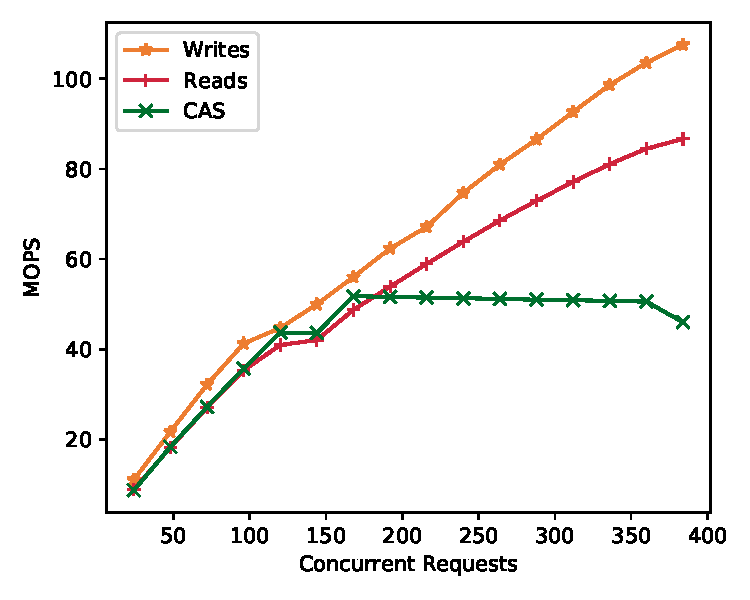
\includegraphics[width=0.45\textwidth]{fig/rdma_concur.pdf}
    \caption{Relative Speed of RDMA verbs as a function of parallel requests}
    \label{fig:rdma_concur}
\end{figure}

RDMA is designed for extremely high throughput and low latency operations. Far
memory systems use their verb library to implement remote memory operations. The
most common are reads, and writes, with the atomic library being used to
implement serialized remote memory accesses. Atomics operations require
significantly NIC memory and are substantially slower than default reads and
writes. Figure~\ref{fig:rdma_concur} Is a benchmark of RDMA verb performance
between two ConnectX-5 NICs. Note that read and write performance are able to
achieve approximately 2x the performance of the atomic CAS instruction.

RDMA atomic operations are known to be slow due to their need to make a PCIe
round trip. In contrast locks held in SRAM require only a few nanoseconds to
perform locking operations. To unlock the full potential of RDMA we convert
compare and swap operations to writes in network. While this operation is
generally unsafe, by resolving all conflicts, and using RDMA reliable
connections, we can ensure all operations succeed and serialization without
using RDMA atomic operations.

\subsubsection{Read tearing}
\todo{place somewhere else}
Async reads and writes can lead to read tearing. Reads
will happily occur on address which are mid write. Writes are done per cache
line, but can span many. To prevent corruption writes are typically followed by
a checksum which provides data integrity~\cite{pilaf,clover}. One advantage of CAS is
that it ensure all reads are complete even if the 64 byte CAS is across cache
lines.

\subsubsection{Memory management hardware}

Hence, a performant far memory system should avoid the use of atomic operations
if at all possible, relying instead on async RDMA verbs.  Even in that case,
existing hardware does provide some guarantees.  For example, RDMA provides
access to memory hosted on a server that likely utilizes a commodity hardware
memory management unit (MMU).  All modern MMUs ensure coherent memory accesses,
and generally ensure a total ordering on local memory requests.  Unfortunately,
due to the complexities of today's multi-core NUMA architectures and PCIe bus
arbitration, it is possible that memory requests may not be serviced in the
order they are dispatched. Happily, the RDMA specification requires that NICs
enforce ordering across operations in an individual queue pair, so sequential
consistency can be ensured by ensuring that all requests for a given memory
location arrive on the same queue pair.


\todo{modify this paragraph so that it is closer to the truth}
Figure~\ref{fig:reorder} shows that this guarantee is actually required: i.e.,
requests across queue pairs are \emph{not} always processed in the order
received in practice.  In this example, we use RDMA \texttt{t\&s} operations to
detect reordering.  Specifically, we generate a sequence of test-and-set
operations that increment the value stored at the indicated location by one if
and only if the current value is as expected, i.e., one lower.  Because we
ensure the operations are delivered to the NIC sequentially, a failed operation
indicates the request was reordered internal to the remote server.  We generate
operations for 1,000 different physical addresses (according to a Zipf
distribution) using a varying number of queue pairs and report the frequency
with which they are reordered with respect to another request for the same
address (i.e., the \texttt{t\&s} operation fails).  As expected, when all
requests are issued on the same queue pair, they are serviced in order.  Once a
non-trivial level of concurrency is reached, however, the reordering becomes
significant, with over 7\% of requests to the same address serviced out of order
when they are spread across 32 queue pairs.\sg{given a zipf distribution, and
16qp around 3\% of packets are reordered. This is detected by checking the
sequence numbers against the known monotonic sequence.}

\begin{figure}[t]
    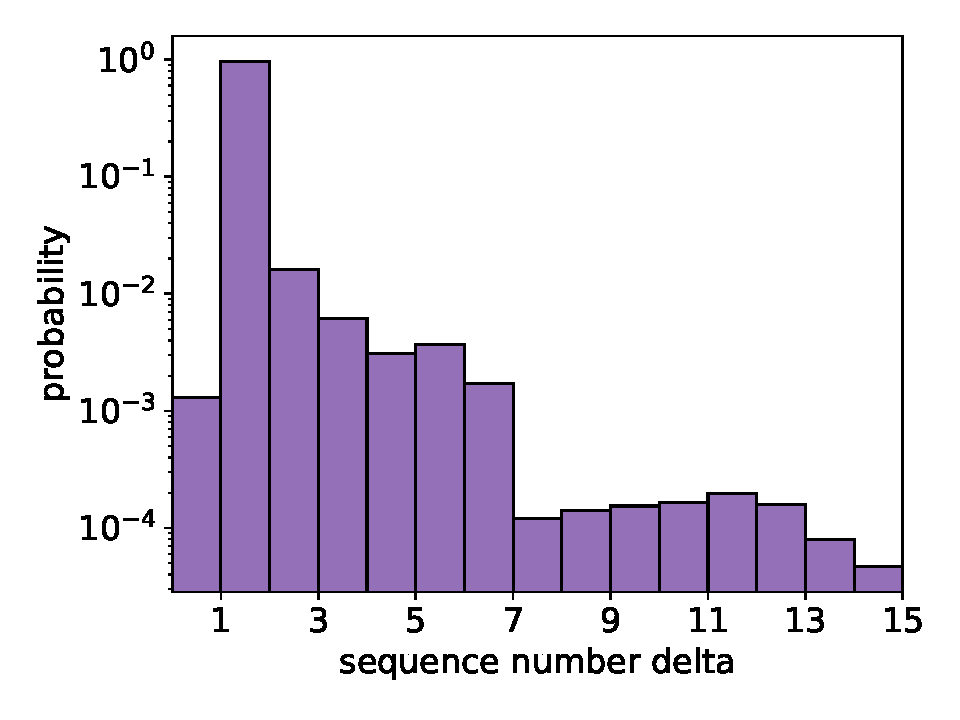
\includegraphics[width=0.45\textwidth]{fig/qp_reordering.pdf}
    \caption{CDF of packet reorderings once QP mapping is applied to a zipf distribution}
    \label{fig:reorder}
\end{figure}

\subsubsection{Queue pair bottlenecks}

 There are two challenges to restricting requests for a given address
 to a single queue pair---one that can be worked around, and one that
 must be addressed.  First, queue pairs are established on a
 client/server basis, so requests from different clients must arrive
 on different queue pairs.  Second, the performance of a single queue
 pair on commercial NICs is significantly less than line rate (likely
 precisely because of the need to enforce ordering constraints).

\begin{figure}[t]
    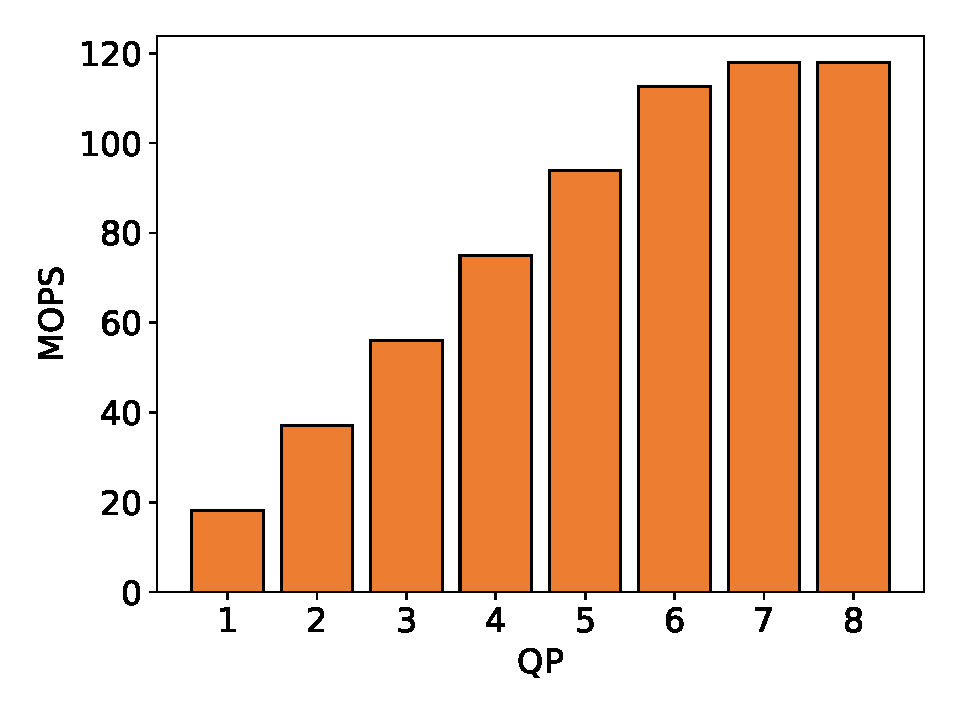
\includegraphics[width=0.45\textwidth]{fig/qp_bottleneck.pdf}
    \caption{Max throughput per QP \todo{take real measurement}}
    \label{fig:qp_bottleneck}
\end{figure}



\subsection{Conflict resolution}

Sharing remote memory creates a variety of performance problems related to
synchronization. Some problems are system, and algorithm specific, while others
are the result of RDMA hardware limitations. 

If synchronization techniques such as spinlocks were naively
implemented the cost of acquiring the lock would be multiplied by many orders of
magnitude. As such developers of remote memory systems typically rely on
optimistic concurrency mechanisms so that in cases were no contention exists
remote operations can succeed on their first try.

\begin{figure}[t]
    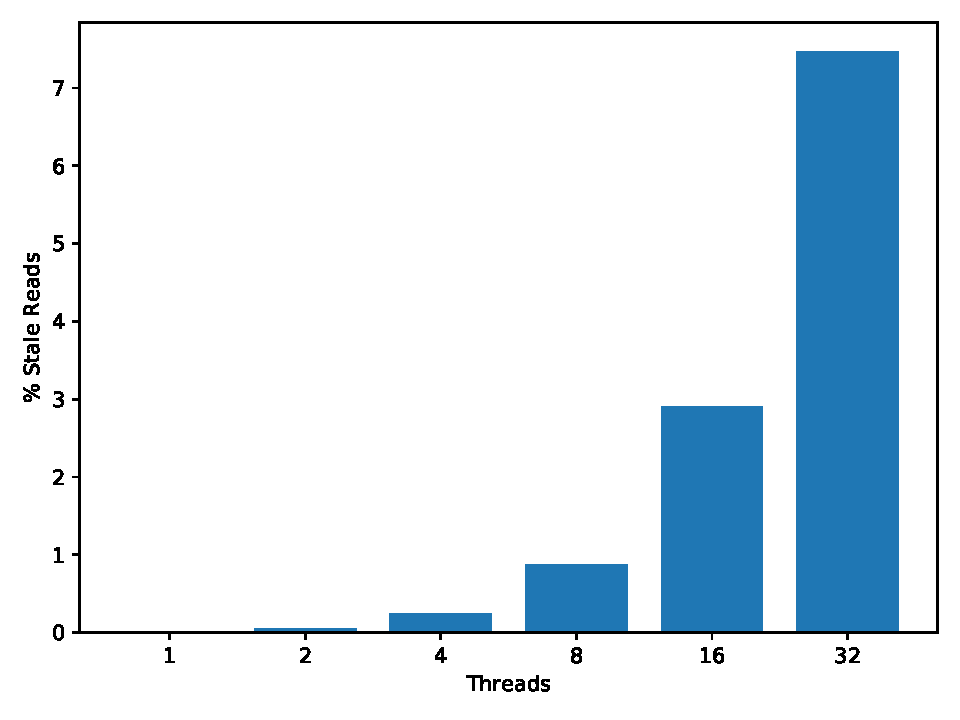
\includegraphics[width=0.45\textwidth]{fig/stale_reads.pdf}
    \caption{Percentage of stale reads made on a 50\% write workload}
    \label{fig:stale_reads}
\end{figure}

Optimistic concurrency algorithms are by definition optimistic, and when
contention does occur their operations must be retried in order to complete the
operation. Clover's opportunistic algorithm attempts to read and write to the
tail of a list for each key, in it's key value store. The location of the tail
of the list is guessed opportunistically (it moves on every write). If the guess
is incorrect the algorithm retries. Both writes and reads can fail, and must be
retried. Figure~\ref{fig:stale_reads} shows the percentage of reads which fail
at a 50\% write workload in clover \footnote{Write fail at a nearly identical
rate}. Retried operations result in large throughput drops (2x) and massive
increases in tail latency (26x) We correct for these opportunistic failures by
caching the location of the most recent writes, and using them to steer
operations from old locations to the most up to date. Ensuring that operations
do not fail drastically improves overall performance under contention. However
some performance is still left untapped as the underlying RDMA hardware has
further limitations. 

\subsubsection{Bandwidth Inflation} 

Optimistic concurrency is designed to have low cost common case operations and
only incur a penalty when conflicts occur. The typical strategy to deal with
conflicts is to arbitrarily determine a winner, and have the loser retry. With
remote memory retires consume network bandwidth and resources. As contention
increases so to does the average cost of each operation. Our results show that
under contention the average cost of read and write operations can inflate by up
to 2x Figure~\ref{fig:bandwidth_reduction} above an optimal O(1) implementation when
all operations succeed on their first try.

\subsubsection{Tail Latency}

High tail latencies are a well understood bottleneck which greatly effect
end-to-end system performance. Under contention optimistic concurrency
mechanisms can exhibit extreme tail latencies. Our experimentation with Clover
shows that under moderate write pressure (50\% write operations with 64 threads)
it's 99th tail latency increases by 83x Figure~\ref{fig:tail_latency}. Reducing the
cost of each operation to exactly 1 attempt can reduce this additional latency
by nearly two orders of magnitude.









\section{On-path serialization}

Given the overhead of remote conflict resolution and the performance
bottlenecks associated with RDMA hardware serialization, this section
discusses how an on-path serializer can dramatically increase
real-world performance by alleviating both issues.  To ground our
discussion, we address both in the context of Clover, a
state-of-the-art far memory system. First we describe how to
effectively do away with the need for most retries by ``fixing''
operations issued with stale hints in flight.  Second, we show how we
can leverage our ability to rewrite RDMA requests after their ordering
is determined to replace expensive compare-and-swap requests with
simple write verbs and rely upon the semantics of RDMA RC queue pairs
to provide serializability.  Additionally, we can leverage this same
functionality to multiplex independent operations across multiple QP
to improve scalability.

\subsection{System overview}

Any asynchronous data structure which allows for lockless reads and
writes must have a mechanism in place to resolve conflicts. When
memory is close, conflict resolution strategies can make many reads
and writes quickly; in the uncommon case of a conflict, the cost of
resolution is typically amortized by the unlikelihood of the conflict
itself. In the case of far memory the cost of a conflict is severe. In
contrast to opportunistic algorithms in a shared-cache architecture,
in a rack-scale disaggregated system conflicts can be detected at the
top-of-rack switch and resolved in the data path. Our solution,
\sword, leverages programmable ToR switches to allow developers with
knowledge of the disaggregated memory protocol to resolve conflicts
transparently in flight as the operations flow traverse the ToR.

\begin{figure}
\center
  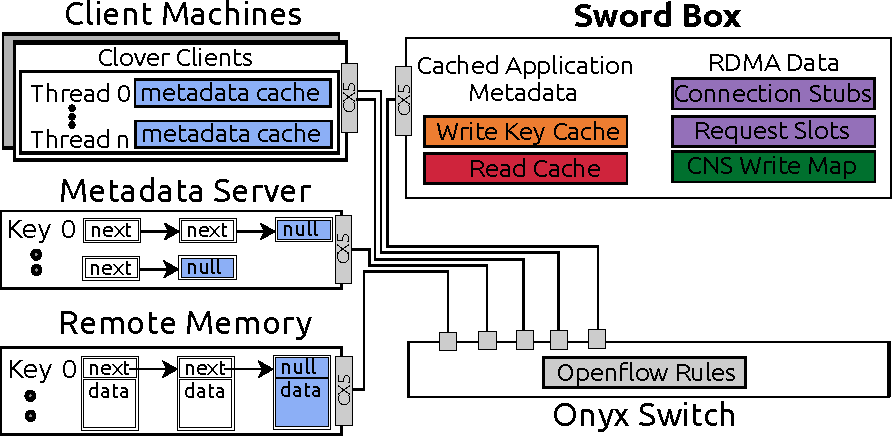
\includegraphics[width=0.45\textwidth]{fig/overview_2.pdf}
  %%
 
\caption{Clients, Metadata and Remote Memory servers are
Clover components. {\sword} is run on a separate server connected to the same ToR.
Routing to {\sword} is effected by adding OpenFlow rules to redirect Clover traffic to \sword.}
%%
\label{fig:overview} \end{figure}

Figure~\ref{fig:overview} shows how {\sword} interacts with the Clover
system.  We envisage {\sword} implemented either as a part of or in-line with
a programmable switch that serves as the top-of-rack (ToR) switch
for all of the memory servers.  Client machines need not be directly
attached to the ToR, although they likely would be in most rack-scale
deployments.  Similarly, the topological location of Clover's metadata
server is irrelevant, but we expect it is also likely connected to the
same switch.  For the purposes of our discussion, we presume that
{\sword} first places all received RDMA requests into a total order
before processing them; likewise responses from a given memory
server are totally ordered before processing.

\subsection{Conflict avoidance}

The single biggest impact an on-path serializer like {\sword} can have
is to dramatically decrease the likelihood of a failed RDMA request due
to a stale hint.  Specifically, because {\sword} can observe and
modify operations as they go by, it can ``correct'' any requests it
knows to be likely to fail.  Note that such replacement is strictly a
performance enhancement---because the requests continue to be
processed by the server as usual, any subsequent reordering will
cause the request to fail (and be retried by Clover), just as
it would have without rewriting.

\subsubsection{Write steering}

Recall that writes (committed with compare-and-swap requests) in
Clover are destined to the presumed tail of a key's linked list, but
the target of any individual RDMA request may be out of date due to
races with concurrent updates.  To prevent such requests from
failing, {\sword} maintains a cache of the location of the most-recent writes
for each key. If a write (CAS request) arrives at {\sword}
destined for a stale virtual address (i.e., an address other than the
one currently cached for that key), {\sword} replaces it with
the cached address.

While conceptually simple, the actual implementation is somewhat
involved due to the design of both Clover and the RDMA protocol and
our desire to remain transparent to both.  Specifically, Clover RDMA
CAS requests do not explicitly specify the operation of which they are
a part.  {\sword} infers the operation by checking the size of the
RDMA request and then extracts the key from the appropriate the
location in the packet.  The key is then used as an index into a
lookup table to find the virtual address of the latest write for that
key.  Our strategy requires only 64 bytes of data per key---the size
of the RDMA virtual address.  Because it modifies the content of the
RDMA request, {\sword} also needs to recompute the RDMA ICRC checksum
to prevent the server from rejecting the request as malformed.

%By
%performing this lookup in the data path all writes succeed regardless
%of how contested the memory address is. \todo{ref fig from words}.

\subsubsection{Read steering}

Reads present a slightly more complicated case. Writes contain the key
to which they pertain---which allows for a table lookup---but Clover's
RDMA read requests only contain the target virtual address and a size.
%When a
%read fails it must be retried, as mentioned earlier reads are
%performed iteratively until the tail of the list is reached, which in
%the case of highly contested keys could be arbitrarily long. Repeating
%reads does not destroy system performance as they are lockless,
%however in terms of client latency each retry adds serious
%latency. What makes handling reads hard is identifying the clover key
%for which the read is for, without additional data in the packet the
%value must be determined another way.
As reads can be for arbitrarily old virtual addresses a naive solution
that stored the lineage of each key would effectively require
caching the entire contents of Clover's metadata server.  Our solution
is to hash the address of each write into an array somewhat larger than
the size of the key space, and store the key along with the address.
Hash collisions are resolved by replacing the old address and key with
the new values, allowing keys with higher update rates to maintain
longer histories in the table. 

When reads arrive {\sword} looks up their destination address in the
table; if the address has a hit the associated key is used to look up
the current tail in the write cache and the RDMA read is redirected to
the cached location.  Should a miss occur---either because the hash
bucket was overwritten by another key, or because the tail address is
not cached---the read is left unmodified.  If it fails to arrive at
the current tail, Clover's default recovery mechanism kicks in and
performs a lookup to the metadata server for the last known address
and the process repeats. We find that by using an array size of
3$\times$ the vast majority of reads succeed first try. One advantage
of this technique is that it is a generalized cache for recent RDMA
reads, and requires little computation to maintain a hot cache. For
performance reasons we forgo heavyweight hash functions and use
the \texttt{murmur3} bit scrambler to attain an approximately even
hash of virtual addresses in only a few cycles.
%---which can likely be
%implemented on programable switch hardware.

\subsection{Enforcing ordering}

The combination of read and write steering dramatically improves the
performance of Clover (as shown in Section~\ref{s:results}), but only
scratches the surface of the potential improvements for far memory
systems.  In particular, if {\sword} is able to ensure that
requests will not be reordered between when it operates on them and
their arrival at a memory server---because, for example, it is
directly connected over a single link---we can leverage the ordering
semantics provided by RDMA queue pairs to completely eliminate data
races.  In that case, there is no need to incur the expense of RDMA
atomic requests; {\sword} can simply replace them with lightweight verbs
to dramatically increase the scalability of a given memory server.
Importantly, this optimization can be applied selectively to only the
set of servers (or keys) for which {\sword} is suitably located
and sufficiently provisioned to manage; Clover operations destined
for other servers and/or keys can be left unmodified---or subject just
to read/write steering as appropriate.

\subsubsection{Connection remapping}

Our key insight is that if all operations---across all client
connections---that share server state are vectored to the same queue
pair, RDMA's ordering semantics will provide sufficient serialization.
In general, the determination of which operations share state is
application specific and requires inspecting each packet, extracting
the relevant pieces of metadata, and vectoring the packet to the
correct connection.  In the particular case of Clover, it suffices to
identify RDMA requests that correspond to requests to read or write
the same key.

%%While removing locking operations is a general principle here we consider a
%%solution for RDMA.  %Different transports with different ordering guarantees
%%would require bespoke solutions.  

The challenge, of course, is that the RDMA specification stipulates
that each client establish its own queue pair with a given server, so
operations for a given key from different clients will arrive on
separate queue pairs.  \sword, then, must interpose on the
full set of queue pairs terminated by a given (set of) server(s) and
vector operations to queue pairs accordingly.

\paragraph{Sequence-space stitching.}

Multiplexing and demultiplexing RDMA requests across established
connections requires a significant amount of care. Requests on a
single connection must have monotonic sequence numbers from both the
sender's and receiver's perspectives. If monotonicity is broken, the
NIC will invoke an expensive go-back-$n$ protocol or issue explicit
congestion notifications. To ensure monotonic sequence numbers on
shared connections {\sword} tracks the outstanding sequence number per QP and
injects the appropriate sequence number into the packet after the
mapping decision has been made.  (Ironically, there is no need to
ensure any particular ordering among requests from separate clients, so
any total ordering suffices.)
%% This monotonic sequence number increment and QP mapping is the
%% serialization point which replaces the use of the RDMA CAS
%% request. As long as a packet is given an atomically incremental
%% sequence number from our middle box and placed on a stateful
%% partitioned connection, it will execute in the same serialized
%% order as if it were protected by a CAS. We are guaranteed this due
%% to the ordering requirements of RDMA reliable connections.

When an RDMA request arrives at {\sword} from a client, it is
mapped to the appropriate queue pair for the relevant key and a
\emph{stub} is stored to aid in mapping the request back, much like a
network address translator (NAT). The stub keeps track of the original
request's sequence number, IP address, MAC address, and queue
pair. Stubs are stored in an array of size $n$ indexed by their
sequence number$\pmod n$ to ensure $O(1)$ lookup when demultiplexing
the response.
%%
In addition to sequence numbers, a \emph{message} sequence number
is used as an RDMA optimization by the memory server NIC. This value
is transmitted as part of the RoCE BTH+ header in the response packet
and corresponds to the highest request number the server has
processed. If this value is wrong in the response packet from the
perspective of the sender (i.e., is less than another message sequence
number previously received by that client), the entire request is
retransmitted.  {\sword} maintains the message sequence number each client
expects to see by keeping track of the number of requests a client has
issued and adding it to the value of the original message sequence
number for that connection.

\paragraph{Request coalescing.}

As an additional complication, {\sword} must deal with the fact
that RoCE coalesces some ACKs as an optimization.  In particular
multiple RDMA requests can be acknowledged by a single
acknowledgment, in the form of either an ACK, ATOMIC ACK, or Read
Response. This occurs when multiple RDMA requests are processed
concurrently.  Because {\sword} maps requests across connections, some
coalesced acknowledgments may need to be disaggregated from the
clients' perspectives.
%
%A final additional challenge in mapping
%requests, is that receiving NICs can coalesce acknowledgment messages. Given a
%single connection, if two concurrent writes are issued, it is perfectly valid
%for an RDMA NIC to only ACK the second write. This is a challenge when mapping
%requests as a coalesced message might have been for a different sender. In our
%scheme as all requests have mapping stubs stored in the middle box,
{\sword} can detect such conditions by comparing the
acknowledged sequence number to that stored in a client's stub; when a
request is coalesced a gap in the sequence number is observable. In
this case we generate the needed acknowledgment at {\sword} and
insert it into the queue pair.
%While read, and CAS requests can not be
%coalesced, CAS requests mapped to writes can be. In the case of
%coalesced ATOMIC ACKs an atomic ACK is generated in place of the
%coalesced write ACK.



\subsubsection{Atomic replacement} 

Once any potentially conflicting operations are mapped to a single
queue pair, {\sword} is free to replace atomic requests such as
compare-and-swap with lightweight alternatives.  From a RoCEv2 perspective
the per-packet transformation from CAS to write can be applied easily
in the data path.  RoCEv2 CAS and write headers only differ by a few
fields. CAS can be thought of as a special case of a write, where the
write is conditional and the length is preset to 8 bytes.
%%

{\sword} transforms CAS requests to writes by modifying their headers: it
switches the RDMA OP field of the CAS to write, copies the CAS
value to the write payload location, sets the DMA length of the write
to 8, and shrinks the IPv4 length value by 4.  Post modification the RoCEv2
and IPv4 checksums are recalculated.
%so the modified packet will not be
%rejected by the memory side NIC.
The transformation from CAS to write
is deterministic and only requires a few cycles to transform the
header.

On the memory server, the NIC processes the write and responds with a
regular, write ACK. Once the ACK reaches {\sword} we apply the
inverse transformation from the ACK to an Atomic ACK which the sender
expects to see.  RDMA Atomic ACK headers are very similar to regular
ACKs with the only difference being that the atomic contains the
original data from the memory location of the CAS. This original data
is missing due to the transformation so we inject a value which
indicates success to the sender.
%%
This value is application specific; in Clover's case 64 zero bits
indicate success.  In other cases it may be necessary to store the
value in the request stub at {\sword}.

%Transforming CAS to
%write does nothing to disturb the RDMA protocol, as both the sender
%and receiver side NIC are oblivious.  However, the guarantees the
%atomic provides, such as write serialization and the prevention of
%read tearing has been lost. To prevent arbitrary corruption of data
%the serialization point must be placed somewhere else. Our approach is
%to detect conflicts in network, and utilize the in order delivery
%guarantees of RDMA reliable connections to ensure safe and serialized
%requests.



\section{Implementation}

\begin{figure}
  \center
    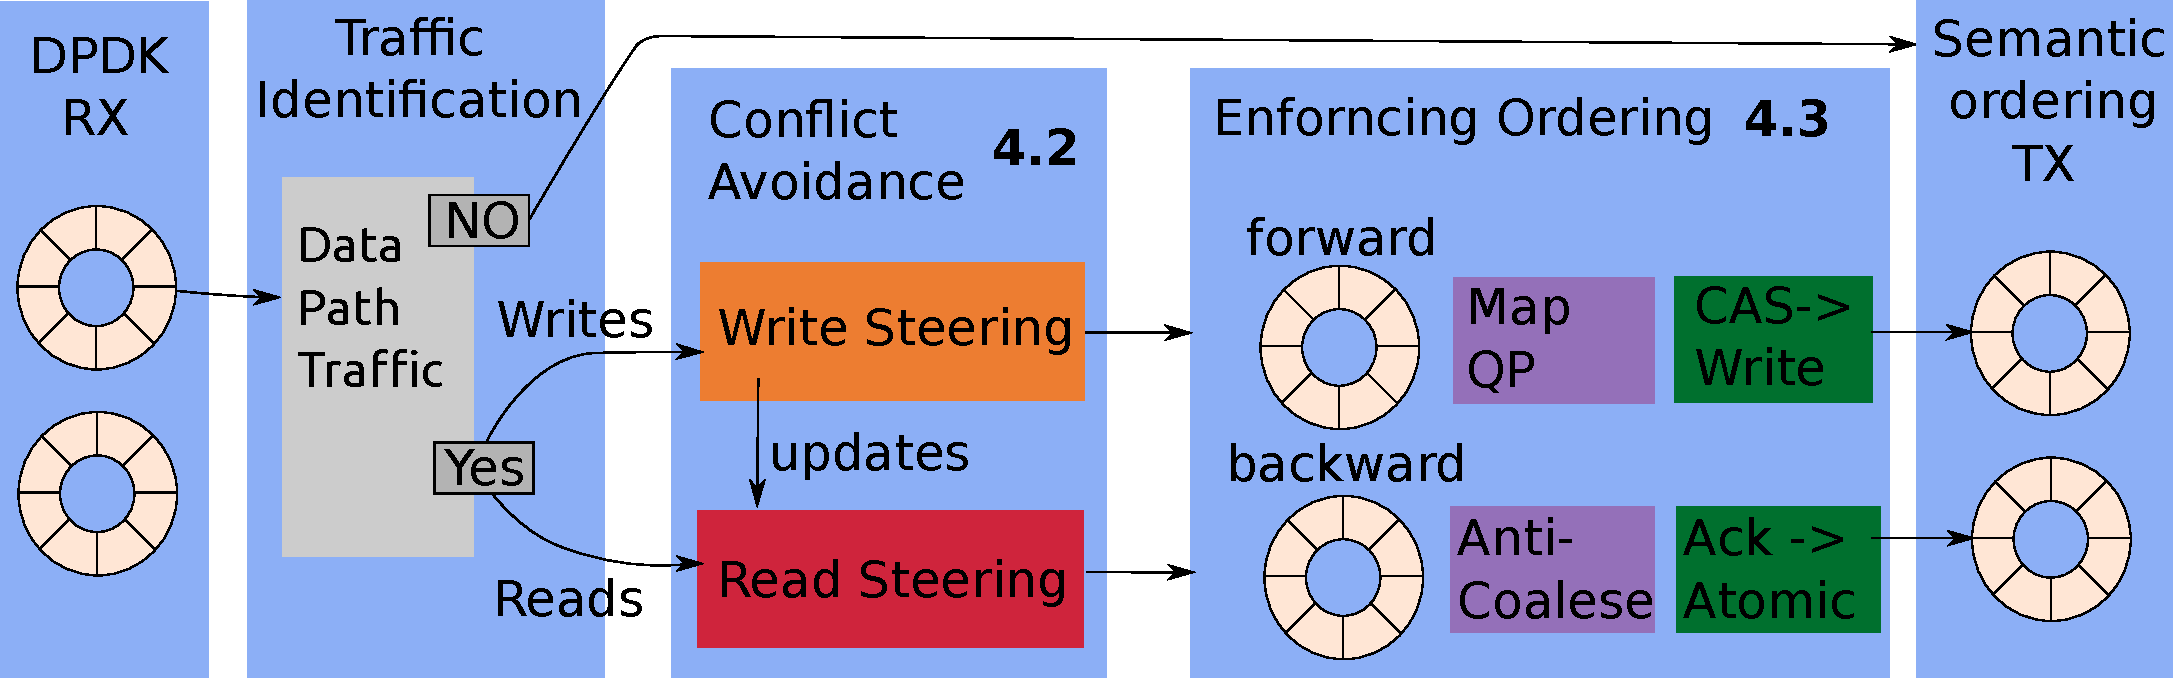
\includegraphics[width=0.45\textwidth]{fig/packet_processing.pdf}
    \caption{\sword's packet processing pipeline}
    \label{fig:system}
  \vskip -0.5em
\end{figure}

Our {\sword} prototype is implemented in P4 and run on a 100Gbps 64 port
programmable switch. Our P4 implementation includes the logic for identifying
and tracking connections, and resolving read and write conflicts in Clover.
Connection multiplexing is implemented separately on a DPDK middlebox discussed
further in this section.

\subsection{P4 implementation}

P4 is a highly constrained language. For example it does not support loops.
Architecturally P4 switches are also highly constrained. Packet parsing must be
performed using the limited TCAM resources available on the switch, conditionals
have a limited branching factor (4). Packets are processed in stages, and device
memory from one stage cannot be accessed at the next, therefore branching
conditionals which access the same variables must be aligned to the same switch
stage if they are to read or write to the same variables. In this section we
describe our P4 implementation of {\sword} and how it adheres to the constraints
of P4 and programmable switches.

\textbf{Parsing} {\sword} has no special requirements for packet parsing. Our
design is focused on RoCEv2 which runs over UDP. Our prototype implements
Ethernet, IP, UDP and RoCEV2 parsing. RoCEv2 headers are required for reading,
and manipulating virtual addresses. One additional header is required for Clover
to read the key out of write requests.

\textbf{Resource Utilization} {\sword} requires SRAM to cache data structure
information. The amount of data required is dependent on the data structure
itself. In clover we cache the last virtual address of each key, and we keep a
cache 3x the size of the keyspace for read steering.


\textbf{Traffic identification} Depending on the disaggregated
rack architecture, memory traffic might be coresident with regular
network traffic.  Additionally some of the traffic on the memory bus
may not require tracking or manipulation. In the case of Clover we do
not interpose upon or modify traffic to the metadata server as it is
not in the read/write path. The first stage of our packet-processing
pipeline classifies requests for manipulation. In our design operators
submit a filter as part of their configuration to allow traffic which does
not need to be modified to flow freely.

\textbf{Dynamic connection tracking}
 A key goal of our approach is to support
serializer-based performance enhancements without modifying the far memory
system itself---including requiring any explicit negotiation with the
serializer.  We add and subtract RoCE connections to {\sword}'s management
tables based upon the send and receipt of CAS operations. The QP and sequence
number for the CAS are stored on send, and the ATOMIC ACK is used to obtain the
other recever's QP.  As this approach requires only a single packet, requests
can be added and removed from our algorithm dynamically with little effort.

%For instance is designed to deal with memory operations made to the wrong
%location via iterative pointer chasing. We strongly suggest that disaggregated
%algorithms take this approach as our middlebox solution only acts to acclerate
%operations in the common case.
\textbf{Initializing connection mapping}
\sg{dpdk only}
As some state may be dependent on the number of connections (such as the
key-to-QP and lock-to-QP mappings), state transitions either require a lock, or
the copying of current state over to a new epoch when new connections are added.
In all of our experiments only one such transition is made. We begin our mapping
after a specific number of clients for the experiment have connected. Once the
total number of clients have connected, a switch is flipped, and the QP
multiplexing algorithm begins. Requests which do not have mappings stored, but
were in flight during the flip have their sequence numbers and MSN values
applied to the connection state of the new epoch.

%\subsection{Operation caching}
%\label{sec:operation-caching}



% \begin{figure}
%     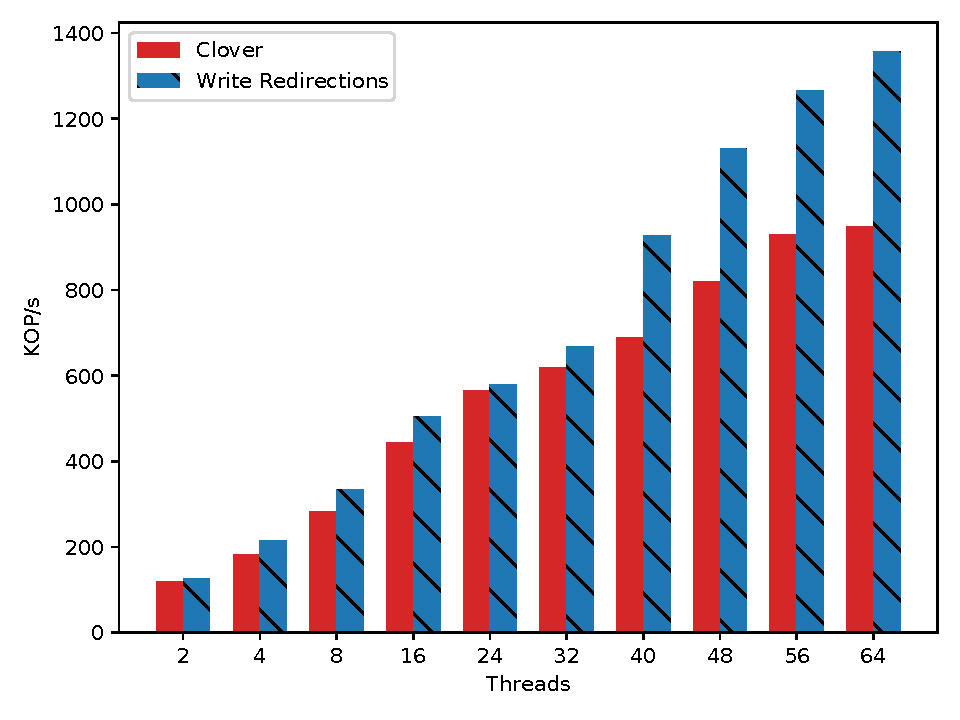
\includegraphics[width=0.45\textwidth]{fig/throughput.pdf}
%     \caption{Default Clover throughput vs. Clover with write conflict
%     detection and correction turned on \todo{recompute with the read caching values (old)}}
%     \label{fig:throughput}
%     \vskip -1em
% \end{figure}

% \subsection{Implementing Atomic replacement}

% In the
% following subsections we describe the dangers of removing atomics, and present
% our solutions.

% A few assumptions must be made in order for this replacement of operations to be
% made. First and foremost all operation serialization must be made, and finalized
% at the point where the CAS is swapped out. More formally, all of the data
% structure invariants which required locking, must be satisfied at the time of
% transforming the packet. Further the order of operations must be maintained
% downstream from the checking of the invariant. These two requirements influence
% the design of any system which aims to make this performance improvement.


%% ACS - This is just lifted from WORDS; no need to repeat here

%% \begin{figure}
%%     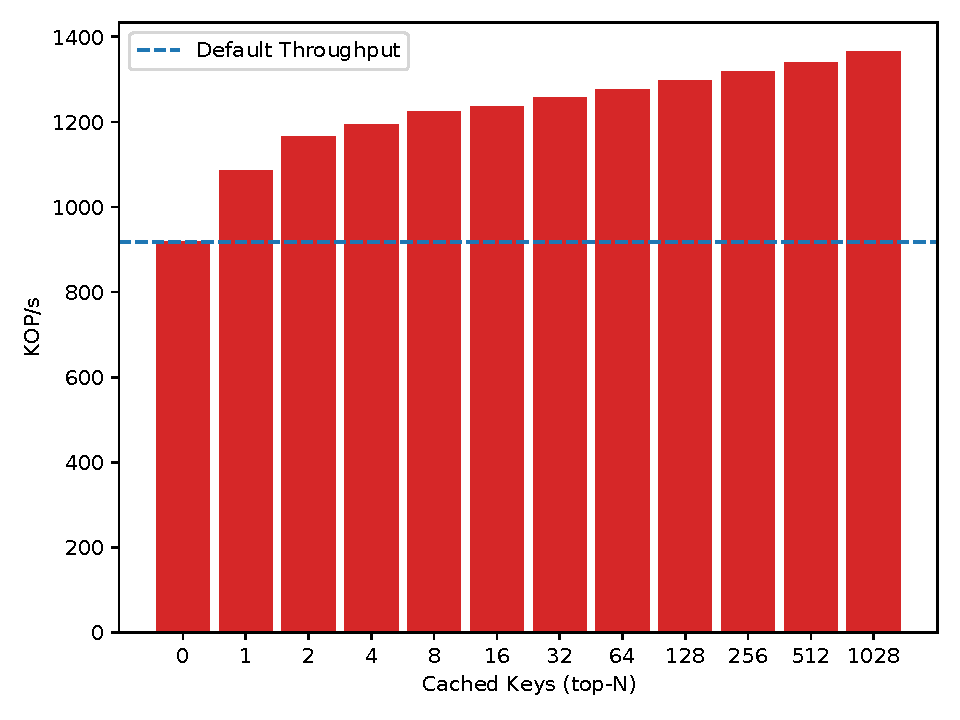
\includegraphics[width=0.45\textwidth]{fig/cache.pdf}
%%     \caption{Performance as a function of keys cached. Caching a few
%%     of the top-$N$ keys provides the greatest marginal throughput
%%     benefits.}
%%     \label{fig:cache}
%% \end{figure}

%% \textbf{reduced cache size} we show that if hot keys are known we require only a
%% small amount of in network state~\ref{fig:cache} we have considered dynamic
%% approaches such as LRU which would allows for a finite amount of space and an
%% arbitrary number of keys to be serviced.

% The first requirement, that the structural invariants
% of the data structure be maintained at the point of transformation demands that
% all of the state required to check the structural invariant be present at the
% point in the network at which the swap is made. This fact increases the memory
% cost on a switch, however with intelligent data structure design the cost of the
% required metadata can be mitigated. In the case of Clover, while each key has
% an entire linked list history that can potentially span megabytes, the only
% required metadata to make the change from CAS to write is the location of the
% tail pointer. In this case the metadata cost is O(n) as it grows linearly with
% the keyspace.

% \textbf{2) reordering} The second requirement, that operations not be reordered
% after the invariant has been checked requires more care in real systems. For
% instance in an RDMA system with two clients, both could have contesting CAS
% operations swapped with writes. As the two clients are transmitting operations on
% separate QP, and the receiving NIC makes no guarantees about ordering between QP,
% the operations could easily be reordered. In the case with CAS, the order could
% be forced by ensuring that if one write was to succeed the second would fail.
% Without this guarantee the preservation of operation ordering must be maintained
% in another way.

% \subsection{Connection Remapping}


% Our solution here is simple, given that we have the key's for reads and writes
% (Section ~\ref{sec:operation-caching}), all operations for the same key are
% mapped to the same QP.  This algorithm requires that a few pieces of state be
% maintained per connection.  First the sending and response QP for each sender
% and receiver need to be tracked. Second the sequence number of each connection,
% and the original message sequence number offset must be maintained. Per client
% connection the pair of QP's require 48 bits, and the sequence + message sequence
% require an additional 48 for a total of 12 bytes per connection. The storage
% requirement for mapped requests varies based on the algorithm. If clients are
% able to issue an unbounded number of async requests, then a buffer large enough
% to maintain backwards mappings for each request is required. In clover clients
% can issue up to 2 async requests, so we keep a two 6 byte mappings for each
% connection available to map back. 

% Depending on the algorithm and the QP mapping scheme requests from a single
% sender can be reordered. That is, if a client makes a read and write request to
% different locations in memory, and they are mapped to different QP, they may be
% returned out of order. Infiniband allows for out of order operations on
% receivers~\cite{infiniband-spec}, which pushes operation ordering to client
% side user space. Roce does not allow for out of order operations. In this case
% the receiving NIC will retransmit if requests are delivered out of order. Here
% we buffer requests in network, as we have application knowledge the size of the
% buffer is bounded (to the size of a single read packet in clovers case). We
% suggest that given the tight memory restrictions on middleboxes algorithms which
% have an unbounded number of async requests leave the ordering of remapped
% requests to client side user space using IB verbs or a different transport layer
% entirely.

\subsection{RDMA ICRC}

RDMA requests are not intended to be modified in flight, and care must
be taken not to corrupt them. RDMA invariant CRCs (ICRC) are
calculated at the time of sending and are designed to ensure the
integrity of the payload. When we modify requests their ICRC must be
recalculated or the packet will be rejected by the receiving NIC. Such
an error would cause an extreme performance hit as any dropped packet
triggers a timeout, and go back n retransmission.  FPGA
implementations of RDMA ICRC have been built in the
past~\cite{Mansour_2019}; the required CRC calculation is identical to
Ethernet CRC, with some additional \texttt{crc32} for the
calculation. This algorithm is highly optimized for general case CRC
calcuation.

Recalculating the CRC for modified requests is the primary overhead of {\sword}
as it must be recalculated after a squence number update, which occurs on all
multiplexed and demultiplexed requests. This overhead could be reduced by either
removing the need for the CRC (which is not a feature available on CX series
NICs) or by allowing an alterative, lightweight checksum which could be quickly
updated based on changes made to the packet while in flight. While these options
are not currently available we believe that commodity switches and SmartNICs
could leverage hardware offloads to reduce the cost, as the CRC calculation is
identical to Ethernet with only the additional need to mask RocE specified
packet felids.

We implemented RDMA ICRC in our DPDK prototype. To our knowledge no P4 switches
have native RoCEv2 support, while some projects have demonstrated that it is
possible to implement by hand, it requires many switch resources and adds
complexity~\cite{p4-telem} we forgot the additional complexity and turned off
ICRC checking on our CX5 NICs similar to prior work~\cite{switchml}. In the
future we hope that RoCEv2 checksums, like TCP, UDP,and Ethernet checksums can
be made hardware primitives on programmable switches.

\subsection{DPDK considerations}

{\sword} is implemented in DPDK for ease of programmability, but
requires that all requests are processed without the aid of RDMA
hardware on the NIC. Using DPDK introduces issues in terms of
performance as individual cores on the server have low packet
processing capabilities relative to dedicated networking hardware. As
such our design is multithreaded and requires the use of careful
atomics for performance.  Our design partitions cores into TX and RX
groups. RX cores are configured via RSS and perform traffic
identification, write steering and mapping. We completely removed the
need for any explicit locking between cores and share as little state
as is theoretically possible. Each TX core serializes requests by
making atomic fetch-and-add updates to a shared region of memory
containing connection sequence and message-sequence numbers. RX cores
are handed packets from TX cores using DPDKs lock-less ring
library. TX cores check packets to determine if they require CRC
computation and calculate the CRC only if the packet has been
modified. Adding a packet handoff between TX and RX increases latency,
however the head-of-line blocking incurred by having a single core
perform both mapping and CRC calculations is too high for our purposes.

We find that by using an array size of
3$\times$ the vast majority of reads succeed first try.
%One advantage
%of this technique is that it is a generalized cache for recent RDMA
%reads, and requires little computation to maintain a hot cache.
For
performance reasons we forgo heavyweight hash functions and use
the \texttt{murmur3} bit scrambler to attain an approximately even
hash of virtual addresses in only a few cycles.
%---which can likely be
%implemented on programable switch hardware.

\subsection{DPDK vs P4}

{\sword} is implemented in P4 and run on a programmable switch, however its
connection mapping functionality is only implemented in DPDK due to hardware
limitations on the programmable switch, and on ConnextX-5 NICs. In this section
we describe why the space and logical complexity of tracking outstanding
requests, and reversing the effects of ACK coalescing is prohibitively hard on
current hardware and suggest small hardware modifications which would make the
implementation simple.

\textbf{Connection Mapping:} Connection mapping requires the storage of a 64 bit
mapping entry for each in flight request (old\_seq, new\_seq, conn\_id,
cas\_to\_write, opcode). These map entries are space concern on programmable
switches. Mapped entries are stored per connection. When an request is mapped to
a connection the entry is generated, when a response returns the entry is
removed.In the worst case, any connection may need to store outstanding requests
for the total number of connected clients as each client could asynchronously
issue a request for the same lock concurrently. 

We use connection sequence numbers to look up requests as they are unique for
each connection, have no collisions, and only require an offset for lookup
($sequence\_number \% max\_clients$). The programmable switch requires that all
storage be allocated at compile time, so we need to provision for the worst case
scenario.  The space requirement grows $O(n^2)$ with the number of clients as
each connection must be statically allocated with enough space to handel a worst
case burst.

Given static allocation if we want to support 512 client threads (the order of
our experiments), in the worst case we need 1024 * 1024 * 8 bytes of connection
storage. 8MB is not much storage, but on our Tofino switch this represents 1/4
of the total SRAM assuming the compiler packs requests perfectly. Unfortunately
this is unlikely the case.  Making this mater worse is that much of switch
memory is allocated into 8 and 16 bit registers. Only a few are allocated to
read and write 32 bits. 2 pipeline stages are the minimum for connection
remapping storage. In the worst case (using 8 bit registers) 8 are required (an
entire pipeline). While expensive this is not a prohibitive cost to
implementation.

We could use a hash table shared by all connections as a lookup for mapping
entries using the key $concat(qp\_id,sequence\_number)$ which would conceptually
reduce the space complexity. However if a collision occurs the collision lookup
must be done in a following stage of the pipeline. This increases the space cost
by the size of the longest collision chain. It also increases the size of each
entry from 64 to 88 as the original queue pair id must be stored alongside the
map entry to detect collisions. This requiring 3 stages to store. Detecting a
collision requires an additional stage to run a conditional statement on the
queue pair id. A chain of 2 collisions therefore would require 8 stages -- our
entire egress pipeline to resolve. Given that we are processing millions of
packets per second on a maximum sized hash table of 16k entries, collisions of 3
or more are common.

\textbf{RDMA Coalescing:} Our greatest unmet challenge with connection mapping
in P4 dealing with RDMA coalescing. When a response is mapped back to a client
it may be a coalesced response, if so the prior map entry must be checked and an
ack generated for that entry. This is an iterative process as a single response
can have coalesced many other responses.

In dpdk this search and packet generation implemented in a 3 line function with
a for loop. In p4 it this functionality was prohibitively difficult to engineer.
The complexity is caused by the need to both search multiple entries of the
outstanding connection list which is not supported by P4 table lookups. In P4
each stage of the pipeline holds unique data and supports a single lookup of the
specified register size (8,16,32), as such we are unable to look up a variable
number of requests to generated coalesced ACKs.

One option would have been to duplicate data, so that if a coalesce did occur,
it could be detected by reading duplicate data in the next stage.  The
difficulty is that under aggressive contention the coalescing 10 or more ACKS is
a common occurrence and duplicate stages would be required for each coalesced
response. Given that a 64 bit entry requires two stages duplicating is not an
option as it would easily exhaust all pipeline stages and never guarantee
correctness.

\sg{I don't actually know if the following would work, it's an educated guess:}
Another option is to use packet recirculation. We could duplicate data once, and
perform a look back to the prior entry to determine if it was coalesce and then
generate another packet to handle the handle the coalesced ack. 
%%
Performing this iteratively could generate all the required ACKs. However it
dramatically increases complexity and inverts the order of packet delivery on
the clients.

\textbf{Conditional Complexity:} The final difficulty in implementing connection
mapping in P4 are conditional statements. In P4 architectures branching is
limited. At any conditional a max of 4 paths can exist.  In clover we reduced
the total number of branching statements to 4 for each of the read, write, CAS,
and ACK pathways. Connection remapping requires complex logic and arithmetic for
generating message sequence numbers, storing request stubs across different
register sizes, and detecting, and generating coalesced ACKs.  Separately none
of these issues are enough to prevent the implementation of connection remapping
on a programmable switch. However in concert the P4 complier was not able to
synthesize a program which could fit into our 16 stages of the Tofino 1. Future
hardware such as Tofino 2 and 3 would likely be able to support this
functionality due to having over double the pipeline logic.

\subsubsection{Potential Fixes}

\textbf{Dynamic Memory Allocation:}
Statically allocating 1024 slots for each client is prohibitively expensive as
it grows with $O(n^2)$ due to static memory allocation. The actual required
amount of space is $O(n)$ as that is the total number of in flight requests. If
we could resize our allocations for each connection dynamically (stealing some
memory from under utilized connections) We would be able to decrease our memory
utilization to $O(n)$. This is a trivial task with an allocator and pointers, but
a prohibitively hard task with static registers and single stage lookups.

\textbf{Turn off coalescing} The most complex part of connection remapping is
calculating coalesced ACKs. The fix for this is simple: Turn off ACK coalescing
on the NIC, as it is only a performance optimization. This fix alone would allow
our design to fit onto a Tofino chip.

\textbf{Complex Conditionals} Increasing the branching factor of conditionals
would greatly decrease the complexity of implementing many complex protocol
features. In some cases branching to 4 or more statements would have allowed
lookups in the following stage to be implemented in a single stage rather than
two.

\subsection{Failures}

Our goal is ensure that under failure \sword does not introduce any correctness
issues. Clover ensures end-to-end correctness for packet failures and client
failures. A key difference between default clover, and \sword enhanced Clover is
a change in atomic domain. In clover atomic operations are executed by a memory
side RDMA NIC, in \sword atomic decision are made at the switch. This
introduces a potential for correctness issues if packets are lost between the
switch, and memory server, and if clients fail during such events.

The primary saftey issue introduced by \sword is a broken list. For example if a
list A->B exists and there are outstanding writes C and D. If concurrent
requests connect B->C and C->D but the CAS for B->C fails and C->D succeeds this
creates a broken chain. Subsequent requests will be steered to the disconnected
chain. One option would be to detect chain breakages and ask clients to reset by
traversing the chain from root to tail. While tempting this approach could cause
inconsistancies as clients might read and write data only to be notified of the
link breakage further down the line. As such we task \sword with enforcing
atomicity on lost CAS operations between itself and downstream memory servers.

First we note that RDMA congestion control makes this problem an unlikely
occurrence on a single hop. During testing we never witnessed packet drop
between the switch egress port, and RDMA NIC, however corrupted packets, and
drops could occur.

If a packet is dropped between \sword and a memory servers NIC, the client will
time out eventually and retry the operation. We track the last sequence number
of each client CAS operation, and the virtual address it was steered to. As
clients are closed loop this is limited to 88 bits per client connection. If we
see that a client retries a CAS we steer that CAS to the same location it was
steered to rather than the end of the list.

In the less likely case that during a dropped packet a client dies, and fails to
retry the chain could potentially remain disconnected indefinitely. To remedy
this final case we keep an additional bit set on each client connection marked
to 1 if a CAS has not been ACKd, and 0 otherwise. Periodically, or upon being
notified of a client failure, our P4 control plane checks the state of client
connections and sees if any outstanding CAS operations were never ACKed. If so
\sword generates the dropped CAS from it's connection table information to
reconnect the list.

Note, it is only when CAS packets are dropped from \sword to memory that these
precautions must be taken. Packets dropped prior to reaching \sword, and on the
reverse path after operations are committed, and handled by RDMA's go-back-n and
Clovers recovery mechanisms.

\textbf{Connection Remapped Failures}

Failures are simpler when mapping connections as a dropped message will prevent
subsequent operations on keys mapped to that QP from executing.  RDMA in order
delivery prevents any data corruption from occurring as no CAS further down the
chain will be committed if a prior one fails. Retransmission in this case is
more complex. A single failed packet will require that all in-flight requests
from all clients on that QP be retransmitted. If a single message is dropped, a
following message will trigger a go-back-n response from the memory side NIC. We
propagate the go-back-n message to all clients with outstanding requests using
the same mechanism we use to repair coalesced acks, but in reverse.  Retransmit
requests can be serviced in any order, as none had yet been delivered to memory,
and if any clients die before retransmitting the structure remains safe in spite
of their failure.

One aspect which requires care is maintaining {\sword} state when dealing with
go-back-n. In the case of Sherman, the value of the lock when a CAS is issued is
stored in the request mapping stub. If go-back-n is invoked the state of the
lock is reverted to the value it had just prior to issuing the failed request.


% Steering requests prior to the completion of CAS is safe in most cases while the
% switch is operating correctly and no client failures exist. However in subtle
% cases saftey violations can be introduced if proper measures are not taken. We
% take advantage of the fact that Clover has built in recovery mechanisms. When a
% failure is detected we rely on clover to recover by triggering it's default
% mechanism. By default when clover detects a failure, it traverses the list of
% keys recursively by issuing reads until it finds the new tail.


% \textbf{Cas fails due to not being the tail}
% In the common case B->C will never fail as the switch will steer requests to
% known successful locations. If a successful client request was not routed
% through {\sword} a CAS can return with a failed operation because it was not
% issued to the tail of the list. In this case {\sword} will see the failed
% response and begin by marking the key as invalid. All responses on that key will
% then be changed to failed CAS which will trigger Clovers recovery mechanism.
% \sg{On swordbox we have two options one of which is to examine the failed CAS,
% assuming that it was a correct write that CAS should point to the next valid
% location. Here the switch can simply update its value for the tail of the list
% to the next pointer of the failed CAS}. The second option is to clear the cache
% and then proactively wait for a successful CAS before steering again.

% \textbf{Packet is dropped after Swordbox, and before NIC processing}
% A trickier case in when the CAS operation for B->C is dropped prior to being
% processed by the NIC i.e the packet is dropped due to congestion. Typically this
% will not happen because the NIC generates pause frames before it becomes too
% congested, in our single TOR setup pause frames prevented packet drops due to
% the close loop design of clover. If the drop does occur however it is difficult
% to detect that the chain has been broken. In the common case the client which
% issued the CAS initially will retry. \sg{I did this on the dpdk box} If the same
% request is issued twice {\sword} could attempt to allow the packet to repair the
% broken chain by issuing it again, however this would incur significant buffering
% on the switch to track potentially lost packets. In the case of a retried CAS we
% mark the key a broken and force all clients to retry by marking their next CAS
% as failed.

% \textbf{Packet dropped, client failure}

% If a client's packet is dropped after \sword commits the CAS and the client
% fails before issuing another request, there is no retry to mark the key as
% invalid. In this case we need to refer to a timeout. On each key we keep a 32
% bit register used to mark outstanding requets. Each key also has a counter which
% counts the total number of CAS issued on the key. When a CAS is processed by
% \sword it increments the counter, and then marks a bit in the 32 bit counter
% modulo the packet counter. The number of the request is stored in the connection
% state of the client. When a response comes back on the client connection it the
% bit in the connection counter is set back to 0. When a CAS is issued, if the bit
% in our CAS tracker is set to 1, then a dropped CAS has been identified. In this
% case the key is marked as invalid and clients must attempt to retry the request.
% Out of band the client connections are checked by our control plane, if a rarely
% written key is unacked for a long period of time the key is marked as invalid
% Out of band the client connections are checked by our control plane, if a rarely
% written key is unacked for a long period of time the key is marked as invalid.

% \textbf{Client sends CAS, packet dropped before hitting the nic, and client
% dies/disconnects before retry}

% If a client cas fails, while another succeeds, and {\sword} also fails before
% being able to correct the fault clients the clients could be left in a state
% where some data is detached, and no mechanism which currently exists would
% detect the detachment. Here we suggest that if {\sword} fails clients trigger a
% \textit{read from the start} recovery to ensure that data remains consistent.


% \textbf{Read Steering}

% Reads also represent a tricky case upon write failure. If we use the same write
% tail to steer reads we can end up with inconsistent reads as they may be on a
% detached tail. Assuming that we will not attempt to repair the broken chain by
% inserting a write, the read is invalid.

% We can remedy this by only steering reads to locations that have had their CAS
% acked. This requires maintaining the write ack tail. And will come at the cost
% of performance. under contention.


% \subsubsection{Thoughts}

% \sg{A naive option would be to keep track of uncommited CAS, and then reissue
% them from the switch. This would defer the atomicity to the switch after it was
% effectivly atomicized by the switch. This is the definition of non-soft state
% though.}

% \sg{The key bit is that we can trigger a fault on all future calls to a broken key.}








\section{Evaluation}
\label{s:results}

%We use two distinct prototype implementations to demonstrate the
%potential performance benefits \sword\ can provide.

We use our DPDK implementation to perform a micro-benchmark where we explicitly
manage RDMA connections to remove the atomic operations used by Sherman's
locking mechanism.  We use the P4 implementation installed on a programmable
switch to show the impact of in-flight conflict resolution at rack scale in
Clover.

%We discuss the relative impact of each of our techniques across
%various workloads, and demonstrate that replacing compare-and-swap
%requests with writes eliminates hardware bottlenecks.

\subsection{Testbed} 

Our testbed consists of a rack of nine identical machines equipped
with two Intel Xeon E5-2640 CPUs and 256 GB of main memory evenly
spread across the NUMA domains. Each server is equipped with an
NVIDIA Mellanox ConnectX-5 100-Gbps NIC installed in a 16x PCIe slot and connected to a 100-Gbps ToR.  Our DPDK-based
micro-benchmarks use only three machines: a load generator, a memory
server, and a machine hosting our DPDK implementation of {\sword}.
The load generator is configured with default routing settings---it
sends traffic directly to the memory server.  We install OpenFlow
rules on a Mellanox Onyx switch to redirect the traffic to the DPDK
box.  For the P4-based Clover experiments, we replace the Onyx switch
with an Edgecore Wedge-100 programmable switch running \sword.
%Figure~\ref{fig:overview} shows the layout of our testbed.
We configure one server as a Clover memory server, one as a metadata
server, and the remaining seven as Clover clients.

%\subsection{FUSEE}

%FUSEE is a recent RDMA-based disaggregated memory system
%with similar design principles to clover~\cite{fusee}. Fusee
%is built on RACE hashing~\cite{race}, and uses a one-sided
%snapshot algorithm for replication. Unlike Clover, FUSEE
%manages it's metadata only using one sided operations
%increasing the complexity of its updates. FUSEE is also not
%designed for persistent memory, updates are performed
%opportunistically, and the \textit{first client to finish}
%succeeds in making an update.

\subsection{Atomic replacement}

\begin{figure}[t]
  \center
    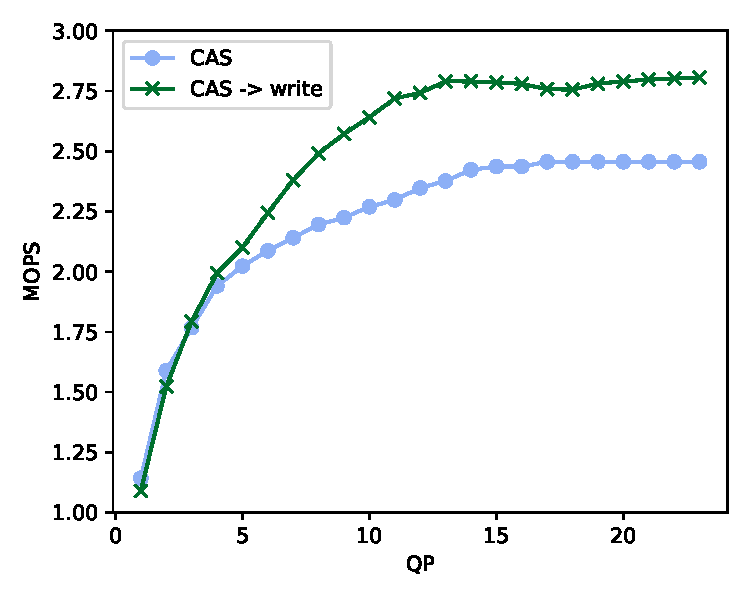
\includegraphics[width=0.99\textwidth]{fig/cas_vs_swap.pdf}
%  \vskip -0.5em
    \caption{Throughput of conflicting CAS and rewritten CAS requests as a function of client threads/QPs.}
    \label{fig:cas_vs_swap}
      \vskip -1em
\end{figure}

\begin{figure*}
  \center
    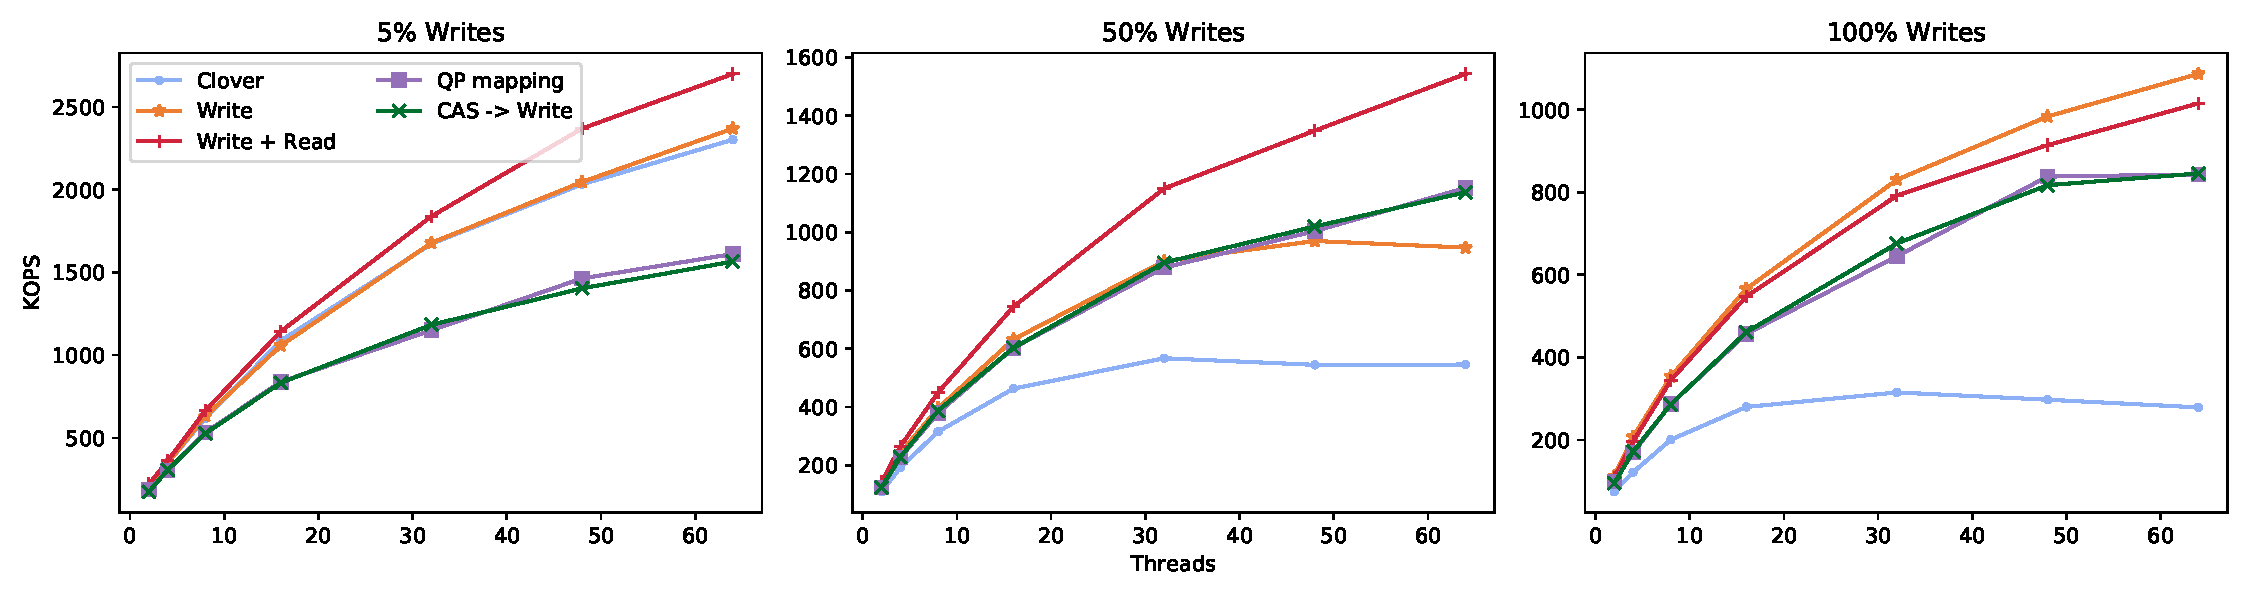
\includegraphics[width=1.0\textwidth]{fig/full_system_performance.pdf}
%  \vskip -0.5em
    \caption{Steering applied to Clover with 128-byte objects across 4 YCSB
    benchmarks. The percentage of workload writes increases from left to
    right. \sword\ throughput relative to Clover is 1.0, 2.8, 32, and 46$\times$ respectively.}
    \label{fig:full_system_performance}
%      \vskip -0.5em
\end{figure*}

We show that \sword\ is able to overcome the NIC hardware
bottleneck by replacing CAS operations with writes
serialized on a given RC by running a micro-benchmark that
focuses exclusively on CAS performance. Specifically, we
extract the CAS request from Sherman's lock operation and
repeatedly generate it from one client to a single memory
server (while routing it through {\sword} using OpenFlow
rules).
%Here we remove clover from the mix and run a simple
%benchmark of RDMA CAS operations between two servers.
%\sword is routed to via a different set of OpenFlow rules.
Each client thread is bound to its own queue pair, and all
client threads issue CAS requests to the same shared virtual
address.  We set the number of cores on the {\sword}
middlebox to 24 so that in our maximal test case each client
thread flows through exactly one middlebox core for the
lowest degree of interference between QP.

%All requests are routed
%through our middlebox.
Figure~\ref{fig:cas_vs_swap} shows the results when all requests are
directed at the same address in the remote server's main memory.  In
the default case (labeled CAS in blue), {\sword} lets CAS requests
flow through without modification, each on their own queue pair.  In
the CAS$\rightarrow$Write (green) configuration {\sword} maps all
client requests to the same QP at the server to ensure serialization
and replaces the CAS operation with a simple write.
%
%all client cores request the same address, and as such all are routed
%onto the same destination QP. Note that this configuration has the
%highest degree of contention for our middlebox as 24 client threads
%must be multiplexed to and from a single client connection. Further
%
%We measure the server throughput in terms of RDMA requests per second as we
%increase contention by adding client threads.
We see a significant increase in performance when \sword\ converts
CAS-guarded requests to QP-serialized writes.  Each configuration hits
a distinct hardware limit: CAS requests bottleneck at the server NIC
due to being applied to a single key
(c.f. Figure~\ref{fig:rdma_concur}).  When converting CAS to
serialized write operations, the bottleneck moves to the DPDK
middlebox.
%cores in our
%DPDK-based {\sword} prototype.
Specifically, DPDK requires all TX for a destination QP to be done by
the same core; hence,
%a specific core on the middlebox. Because of this
%requirement
all requests must flow through a single core, capping the  performance of our
DPDK implementation to the maximum per-core
throughput of our middlebox server: 2.8 MOPS.
%In this configuration all requests to the memory server must be processed by
%the same TX core. As such our bottleneck is approximately 2.8 MOPS. Hardware
%implemented CRC, cache tuning, and better lock management for TX queues could
%yield higher per core performance in the future.
%% Despite this restriction, these results show that replacing CAS with write
%% avoids the memory server NIC's hardware bottleneck, enabling increased
%% scalability with a more performant {\sword}---such as one implemented on a
%% programmable switch. ~\sg{Our limitations here are due to programmability issues
%% on the programmable switch, multiplexing across connections inflates state
%% requirements and makes storing dynamic connection state tricky given only a
%% static number of fixed width registers.}



\subsection{Steering in Clover}

While atomic replacement is feasible, it requires \sword\ to
explicitly manage and remap all the RDMA connections to a given (set
of) server(s)---a resource-intensive task.  Here, we consider the more
general and lightweight case where \sword\ serves as a
performance-enhancing proxy and attempts to avoid failed operations by
steering requests in flight.  We use workloads from the YCSB
benchmark~\cite{ycsb} to access 1,024 128-byte objects stored in Clover.  (Results for a range of sizes are presented in Appendix~\ref{ss:psize}.)
%a
%breakdown of our techniques, mainly read and write caching, QP mapping, and
%atomic replacement with respect to their effect to system
%% performance of four different
%% YCSB workloads. We choose YCSB-B (95\% read and 5\% write) as our baseline, and
%% YCSB-A (50\% read and 50\% write) to demonstrate how our algorithm performs
%% under high contention.  We also show the performance boosts obtained while
%% running a 100\% write workload which is intended to emulate other programmatic
%% workloads which are update heavy.

\subsubsection{Throughput}

Figure~\ref{fig:full_system_performance} shows the impact of \sword's
techniques at various levels of contention.  A read-only workload
exhibits no contention, so \sword\ simply passes through all
operations unmodified achieving a maximum throughput of approximately
40 million operations per second in our testbed.  As a point of
comparison, we also plot (in green) the performance of a
non-replicated instance of FUSEE, in which case their SNAPSHOT consensus algorithm
degenerates to a lock-based approach.  While FUSEE's absolute read
throughput on our testbed is considerably higher than reported by the
original authors on their own hardware, it is less than half that of
Clover on this workload.  While Clover clients can safely cache the
linked-list location for popular keys (because any updates will cause
the next pointer of the returned element to be non-NULL), FUSEE
clients must always issue two seperate, dependant RDMA reads: one to
obtain the current location for the desired key, and then one to read
the value.\footnote{While
the results in the FUSEE paper suggest it outperforms
Clover~\cite[Figs. 13--15]{fusee}, Clover's
client cache is disabled in those experiments, forcing all reads to go through the metadata server.  Moreover, in our experiments, FUSEE fails to scale beyond 256 clients---published results only go to 128~\cite{fusee}.}

%% scaled to
%% 256 clients before it was unable to complete our benchmarks.
%% (beyond what was reported~\cite{fusee}). We compare \sword
%% to FUSEE despite these differences because it is the most
%% recent RDMA-based disaggregated memory system.

Clover (shown in blue) performance
decreases markedly with even 5\% writes, nearly matching FUSEE; write steering
alone (orange) provides minimal performance improvement as
the vast majority of writes succeed on their first try---it
is the reads that are failing.  Steering both reads and
writes (red) restores performance, although to a slightly
lower overall throughput as even successful Clover writes
require two RDMA operations instead of one.
%Individual writes, however, can lead to many stale reads
%immediately thereafter which leads write steering to offer
%a 1.17$\times$ throughput improvement.
%
%Applying QP mapping to the read majorly case adds too much
%computational overhead to give a benefit when writes are
%low, and only a few compare and swap operations exist.
%
At 50\% writes, over half of all write requests fail so
applying write steering almost doubles performance.  The
steered writes, however, then out-pace reads causing the
majority of reads to fail unless \sword\ also applies read
steering.  (The impact on tail latency is clearly shown in
Figure~\ref{fig:tail_latency}.)  Of course, in a 100\% write
workload write steering alone is sufficient.  While FUSEE
suffers less from increased contention, its writes require three
or more RDMA operations; as a result \sword\ pushes Clover to achieve 1.9--2.5$\times$ higher
throughput than FUSEE.


%
%This workload leads to enough common case failures that
%performance overhead of performing QP mapping still yields a
%performance boost.
%
%in the workload.



%%\todo{real takeaways}

% \subsection{Memory Utilization}
% Our techniques give a performance boost at the cost of in network memory. We
% took special care to design our algorithms so that they could 1) use only a
% small amount of network memory, 2) be scalable depending on the resources
% available. We show how our performance varies as a function of the available in
% network state.

% As seen in Figure~\ref{fig:cache} our write caching is able to provide a
% significant performance boost while only using a small number of cached
% addresses. In the following experiment we show the maximum performance boost we
% can provide as a function of the available in network memory. Specifically in
% the case of read and write caching this means shrinking the size of the
% available cache. In terms of QP mapping it restricts the number of connections
% which can have their connections mapped. Unmapped connections must use atomic
% operations for their requests to succeed.

% \begin{figure}
%     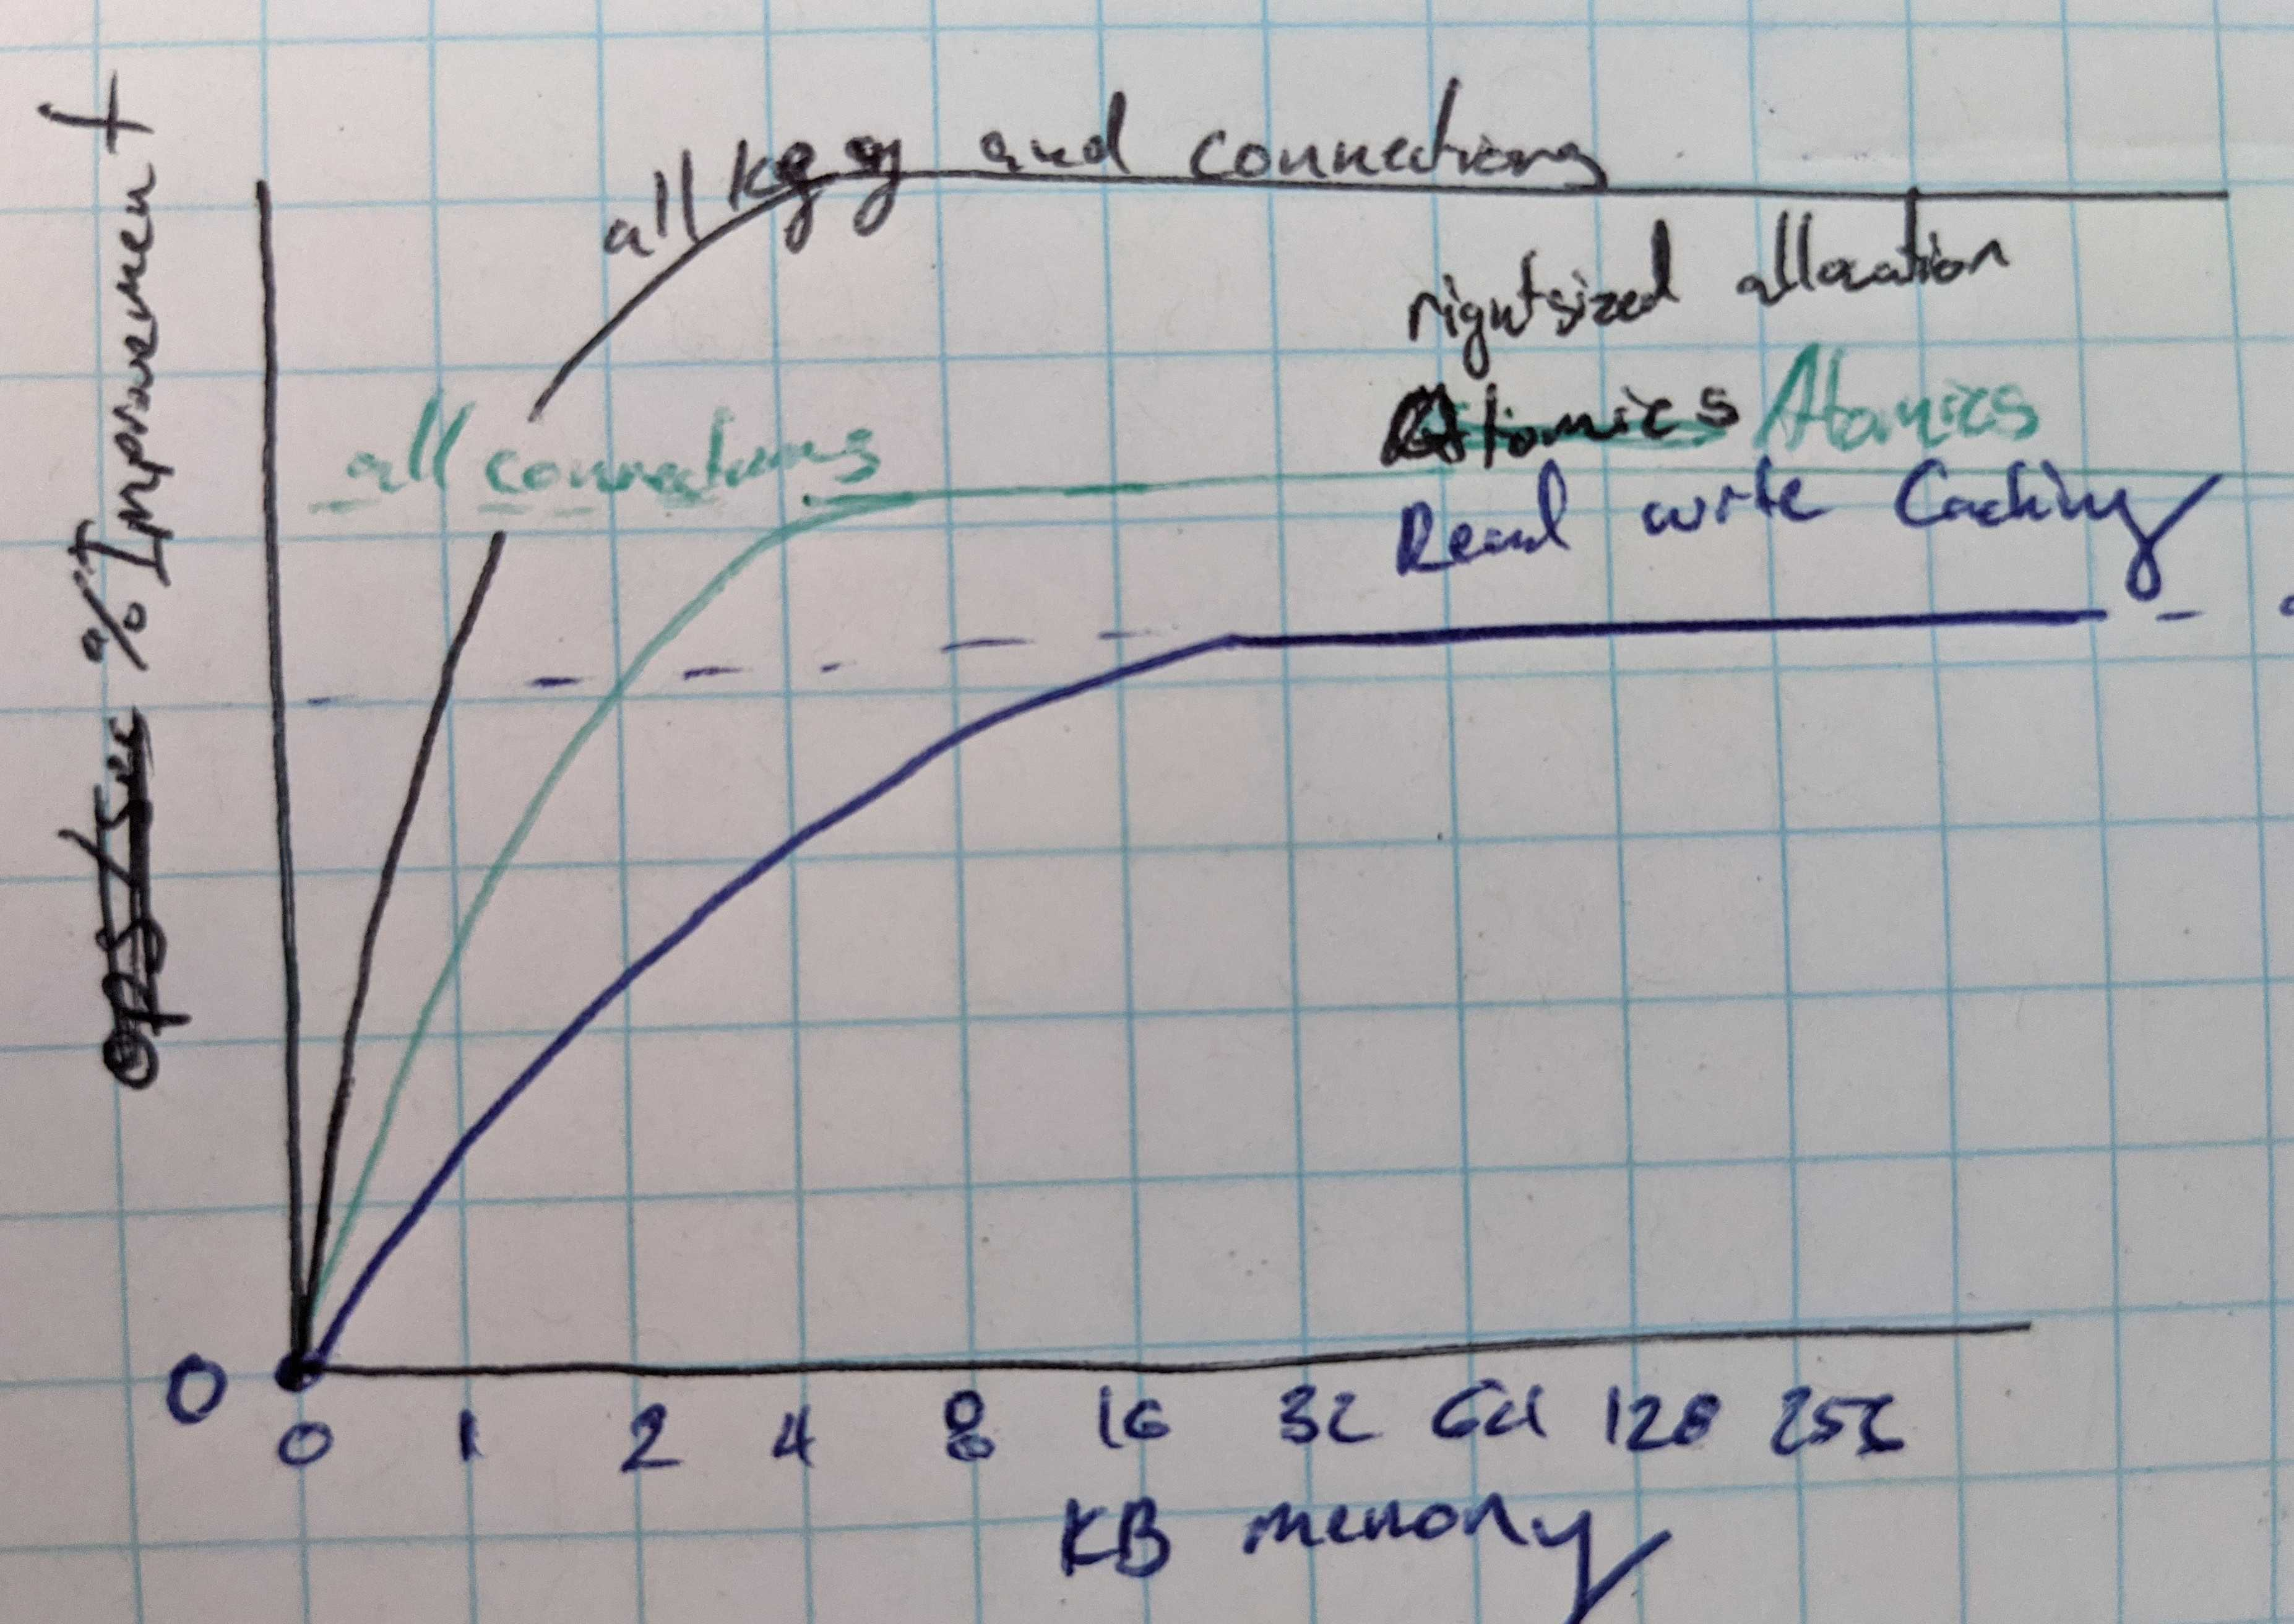
\includegraphics[width=0.45\textwidth]{fig/memory_util.jpg}
%     \caption{{Relative performance improvement of our techniques with restricted amounts of memory. Here a rightsized allocation implies that for the given number of connections we could support, all requests were mapped and reads and writes were cached.}}
%     \label{fig:memory_util}
% \end{figure}
%%\todo{say something real about the the memory utilization takeaways}


\subsubsection{Bandwidth reduction}

\begin{figure}
    \center
  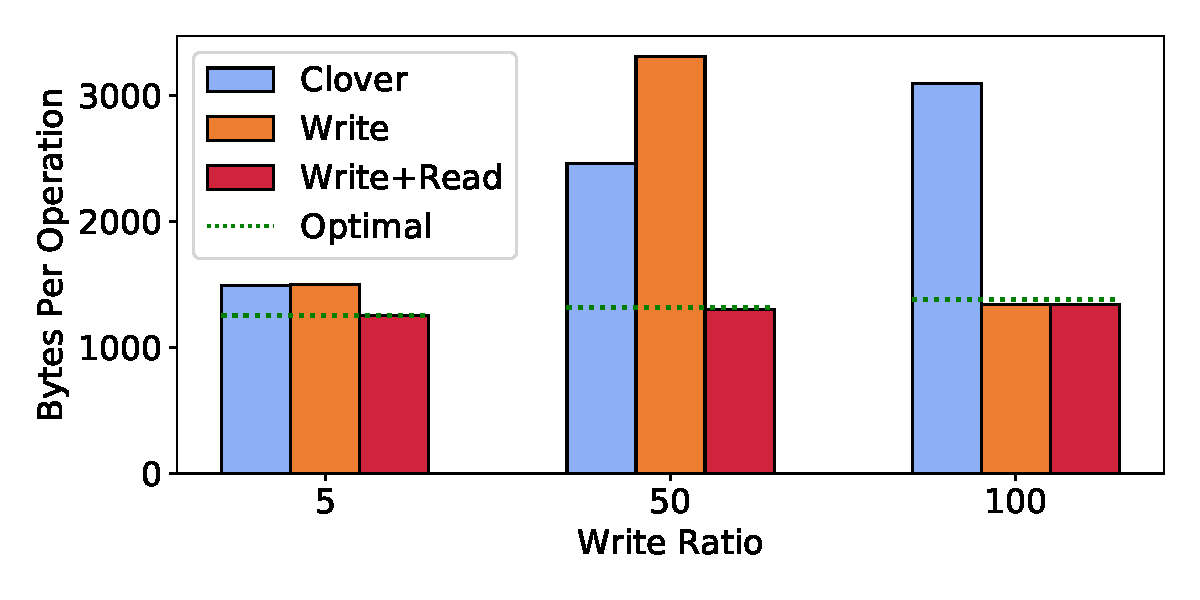
\includegraphics[width=0.99\textwidth]{fig/bandwidth_reduction.pdf}
  \centering
   \vskip -0.5em
    \caption{Average number of bytes required per Clover
      operation on 128-byte objects using each of the three techniques at various write
      intensities.}
    \label{fig:bandwidth_reduction}
     \vskip -0.5em
\end{figure}




%Placing memory operations in-band with regular network traffic can be
%problematic as applications' remote memory usage has the potential to
%vary dramatically per application.
Under contention, Clover's remote operations can require additional
packet exchanges which inflate the bandwidth necessary to service the
same number of memory accesses.  \sword's steering algorithms
remove the need for requests to retry, eliminating the overhead.
%
%Figure~\ref{fig:bandwidth_reduction} shows the average bytes
%per Clover operation under three different workloads for default
%Clover as well as {\sword}'s two steering techniques.
%
%% We calculate the optimal expected cost of a Clover operation by
%% averaging the cost of a successful operation across reads and
%% writes. We get the weighted average by multiplying the cost of a read
%% and write by the appropriate workload percentage. Each write consists
%% of an RDMA write followed by a CAS, along with the responses for each
%% message. A read consists of an RDMA read and read response, and
%% usually an additional metadata read made asynchronously with the main
%% read to fetch the latest position of the tail in case the first memory
%% read fails. Clover performs this second read opportunistically (in
%% around 99 percent of all reads in these workloads), however sometimes
%% it is omitted leading to a small over-approximation in our estimate of
%% ``optimal''.
%
Figure~\ref{fig:bandwidth_reduction} plots the average bytes per
operation for each strategy across the three workloads with writes.
(The read-only workload, not shown, never needs to retry.) We calculate the value
for each technique by summing the total bandwidth across a run and
dividing by the number of operations. Clover's bandwidth usage
increases with contention, growing by 2.5$\times$ at 5\% and
16$\times$ at 50\% writes---all of which is recovered by applying
read and write steering. Write steering alone causes significant
inflation in the cost of operations at 50\% writes because many read
requests fail as discussed above.

\subsubsection{Tail latency}

\begin{figure}
    \center
    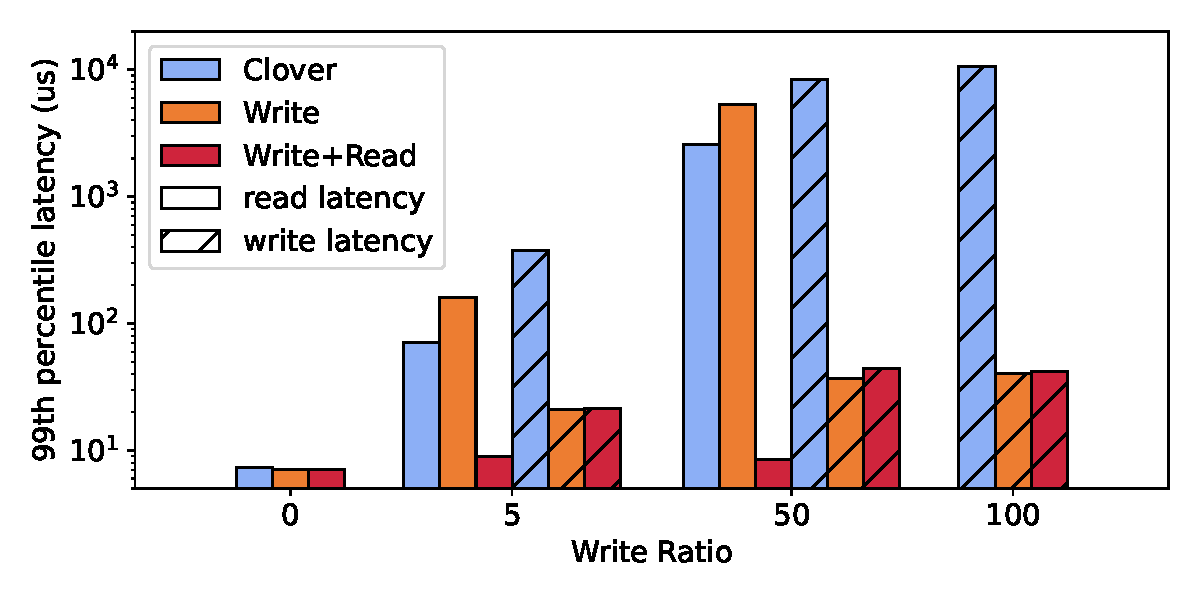
\includegraphics[width=0.99\textwidth]{fig/99th_latency_dense.pdf}
\vskip -0.5em
    \caption{99th-percentile tail latencies of read (solid) and write
      (striped) Clover operations at various write intensities. (Note logarithmic $y$ axis.)}
    \label{fig:tail_latency}
%      \vskip -1em
\end{figure}

%% Perhaps the most critical variable that governs overall system % performance
%is tail latency. In the context of disaggregated memory % systems, reads and
%writes are often deeply integrated into the % computational logic of a program
%and the whole program must wait for a % page fault to complete before
%continuing. We therefore consider poor % tail latency to be a fundamental
%barrier to the widespread adoption of % far memory systems.
Optimistic concurrency is well known to exhibit poor tail latency under
contention, and Clover is no exception.  \sword\ significantly reduces latency
as steering ensures that nearly all requests succeed on the first try.
%
Figure~\ref{fig:tail_latency} shows the 99th-percentile tail latencies
associated with \sword's read and write steering in comparison to default Clover
at varying write intensities. Clover's p99 read latency (solid blue) at 5\%
writes is 70~$\mu$s, around 10$\times$ its baseline our our testbed. With read
and write steering (solid red) the read tail latency drops to 8~$\mu$s---a
8$\times$ improvement over Clover even in this low-contention regime. At 50\%
writes the performance increase from steering increases dramatically: p99 read latency drops by over 300$\times$.
%% As discussed above, in either % case applying write steering alone actually
%hurts performance, as it % makes reads more likely to fail.  % %read
%performance is improves by 2$\times$ % %relative to Clover with the exception
%of write steering alone. When % %write steering is applied without the aid of
%read steering the writes % %quickly out-pace the reads, leading the vast
%majority of reads to fail % %on their first attempt.  % Given that these tests
%were conducted with a % Zipf distribution across 64 cores it is highly likely
%that more than % one thread is writing to the hottest keys at any point during
%the % run. This leads some read requests to fail 10s of times before %
%succeeding.
%
%Because of this property we suggest that read and write steering be used in
%concert unless the workload is explicitly known.
%
Writes (hashed) have slightly more than double the latency of reads as they
require two round trips and atomics are slower to execute than other operations.
Combined write and read steering provides a 17, 189, and 252$\times$ improvement
in write tail latency, respectively, across 5, 50, and 100\% write workloads.
As one might expect, performing write steering alone privileges writes over
reads, dropping their tail latencies slightly further---at the cost of a
dramatic spike in read tail latency.

%% Figure~\ref{fig:tail_latency} also shows the performance of queue pair
%% mapping and atomic replacement (CAS$\rightarrow$Write) when applied in addition
%% to write+read steering.  Because the requests are already likely to
%% succeed, there is no reason to expect any significant drop in tail
%% latency by vectoring the requests to a particular QP or removing the
%% CAS guard.  Rather, these plots show that the (significant) 
%% logic required in {\sword} to implement these functions result in only
%% marginal increase in tail latency relative to steering alone---and still
%% significantly outperforms Clover alone.


%The application of QP mapping and swapping
%CNS to writes does little to effect tail latency as their performance
%cost comes largely as an increase to the average.

\subsubsection{Partial steering}

\begin{figure}
    \center

    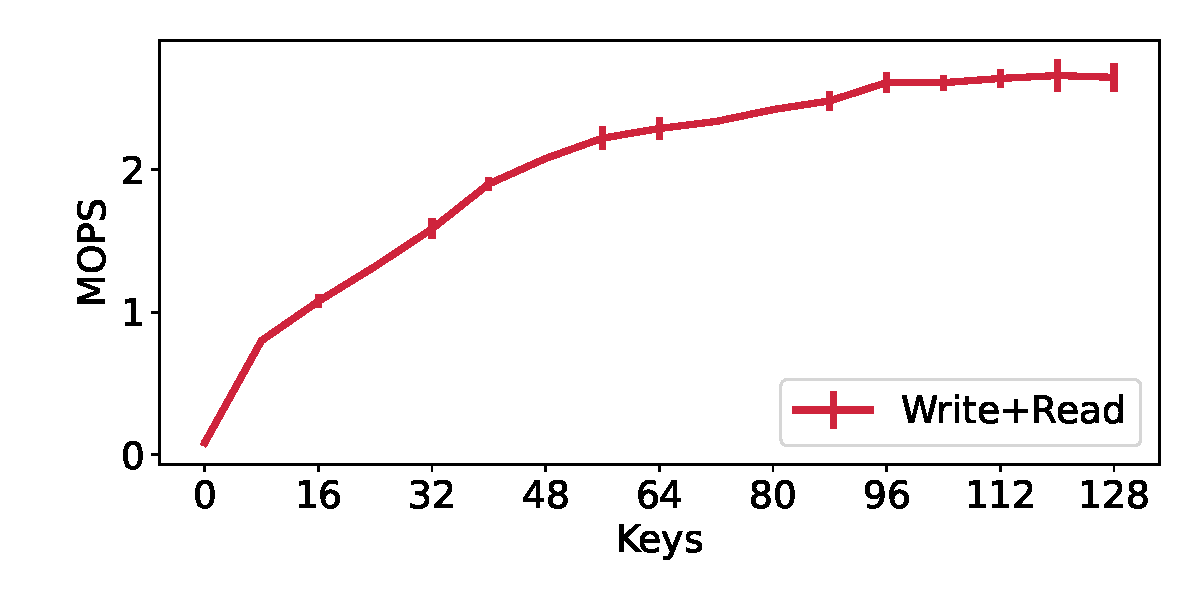
\includegraphics[width=0.99\textwidth]{fig/keys_tracked.pdf}
\vskip -0.5em
    \caption{Per-client throughput as a function of the number of
      Clover keys \sword\ steers.  50:50 workload averaged 
      across 6 hosts each running 56 threads.  }
    \label{fig:keys_tracked}
%      \vskip -1em
\end{figure}

One of most appealing aspects of \sword's steering is the fact that it
need not be applied to all servers, or even memory regions (i.e.,
Clover keys) of a given server.
%In the presence of heavy-tail
%workloads, even steering accesses to a msall number of hot (i.e.,
%highly contended) keys can provide a major performacne boost.
Figure~\ref{fig:keys_tracked} shows per-client throughput as a
function of the number of keys steered by \sword.  To accentuate the
impact, we use a Zipf parameter of 1.5---as opposed to 0.99 in prior
experiments---to enhance the locality of requests.  (See Appendix~\ref{ss:zipf} for a full range.)
%If a programs state is too large to cache on a switch (millions of keys) but a
%few hot keys are highly contested, {\sword} can still provide significant
%benefits by acting on only on the contested state. In the following experiment
%we track a subset of Clovers keys, allowing the rest to flow through
%uninterrupted. In this experiment we run clover at a zipf of 1.5 (most requests
%are on lower keys). We add keys to \sword's tracking list in order of hotness by
Steering requests for only the hottest-8 keys provides a 9.5$\times$
improvement while tracking the hottest 64 delivers
27$\times$.
%; maximum performance boost (i.e., tracking all keys, not shown) is
%(c.f. Figure~\ref{fig:contention}).




\section{Limitations}

The main limitation of our work is that our middle box is developed in user
space software and not on programmable networking hardware. There are additional
limitations, in terms of language restrictions and processing power which occur
on real hardware but not in our DPDK prototype. For example in programmable
switches the need to recirculate packets which exceed the computational capacity
of a pipeline results in decreased overall bandwidth. We use prior work on
programable switches to inform our DPDK prototype and intentionally avoid
decisions which would not be implementable on a programmable switch.

Our experiments fall short of the underlying hardware limits. Our results are
relative and show real performance boots which are obtained by reducing hardware
contention. In future work we would like to extend our measurements to push the
limitations of the underlying hardware. We expect that measuring at line rate
will only increase the benifit seen by reducing this contention based on our
current measurements~\ref{fig:full_system_performance}.

\section{Conclusion}

We leverage the top-of-rack switch to provide cross-client ordering
semantics unavailable in today's RDMA standard, dramatically
increasing performance of systems that rely on atomic operations and
optimistic concurrency.  Concretely, we show that \sword\ can resolve
in-network contention and enable efficient sharing of remote memory
with on commodity RDMA NICs.
%for passive remote memory and show that by resolving
%conflicts in flight,
 Our full-featured DPDK prototype demonstrates the potential of
 removing atomic operations and relying entirely upon queue-pair
 ordering guarantees.  While connection multiplexing is currently
 gated by the single-core performance of DPDK, our P4 steering
 implementation shows order-of-magnitude gains in the context of one
 of the highest-performing systems available.

% Moreover, we describe how it is
% possible to replace atomic memory operations with traditional reads
% and writes to avoid performance limitations inherent in such
% heavyweight operations.

\section{discussion}

In this sections we discuss the limitations, generality, and scalability of our approach.



\textbf{RDMA Failures:}
%%
In our approach the switch updates it's memory prior to the RDMA packet
landing in remote memory. This operation is safe under the assumption that no
packets are reordered after egress from the switch and that all operations
are successful. If a c\&s packet updates switch memory, and then is rejected
by the NIC or endhost a reconciliation of memory must take place. The
signifier to the switch that a failure has occurred is an RDMA c\&s NACK. When
this occurs the switch can dump all of it's soft state and reset. This will
cause the clover protocol to revert to it's default chain walk to learn new
values. Our approach requires only a single successful c\&s operation per key
to rebuild its cache.

\textbf{Read acceleration:}
%%
Our current implementation concentrates of fixing write contention,
however there is no limitation which prevents us from gaining a performance
boost on reads. In future work the same RDMA cache can be used to steer
reads which are issued by clients with stale information.


\textbf{Scalability Implications:}
%%
The advantage of using a TOR is that all operations within a rack can be
serialized. However in many cases this degree of total ordering is not
required. For instance access to a single memory server can be serialized by
performing ordering on a SmartNIC connected to the endhost. Our techniques
could be built into smartnics which would allow for them to scale arbitrarily
under the assumption that writes do not span multiple remote memory machines.


\textbf{Alternative Datastructures}
%%
As noted in~\ref{sec:future} the crux of applying our approach to other
structures is the complexity of the data structures invariants. For Clover
the invariant is simple, all writes must append to the end of the list. To
enforce this invariant the last element of the list must be cached to ensure
that the tail location is known.

The more complicated the structural invariants are to maintain, the greater
the information which must be cached; for example an \textit{ordered} list.
To illustrate the additional complexity of maintaining order consider how
clients could perform inserts. First, like clover, clients could write their
entry to a private memory region. Second two pointers must be written, one
which points to the next item, and another from the prior item to the newly
written one. The client could issue the writes itself, however when the
insert occurs it would need to traverse part of the list to ensure that the
result had been inserted to the correct location and collect a lock on both
the prior and successor items. Enforcing the ordering invariant requires that
the switch cache the entire list.

Ordering is more complex in terms of space to maintain compared to only
appending to a lists tail. The complexity of generalizing our technique to
any data structure being is that the switch must cache all necessary metadata
to maintain a data structures invariants.

We've considered exploring the class of data structures which have either
weak structural invariants, or those which only cost $O(1)$ to check. Additionally some
data structures amortize the cost of operations which require complex
invariants. For instance, rather than storing an ordered list, using a
partially ordered list with fast accesses which can be periodically
transformed with expensive operations to be consistent.

%We are exploring the potential set of future data structures currently. One
%example of a data structure with more complex invariants is a B-Tree. In this
%case ordering must be persevered at each level of the tree, and also some
%operations require that many locks up the tree be obtained. We speculate that
%algorithms used in Clover such as writing to a local scratch space and then
%atomically updating a shared vairable could be used in more complicated
%scenarios as well, such as this.

%\textbf{zipfan 0.75} 
%%
%We chose this because it shows scaling isues before we
%start to hit the hardware issues. There is no good answer to this question.

%\textbf{Why does the switch have to store the last key written per client}
%%
%The last write is not stored. Client writes occur in two parts, a private
%write to their own scratch space, and a commiting atomic c\&s. The write
%which is stored is the outstanding writes, i.e writes which have been placed
%in the local storage, but not yet connected via a commiting operation.











%\section*{Acknowledgments}

\newpage

\balance
\vspace{-0.3cm}
{\footnotesize \bibliographystyle{acm}
%%\bibliography{paper,sysnet}}
\bibliography{paper}}
\vspace{-0.5cm}

\end{document}
